%% example.tex
%% Copyright 2012 Bruno Menegola
%
% This work may be distributed and/or modified under the
% conditions of the LaTeX Project Public License, either version 1.3
% of this license or (at your option) any later version.
% The latest version of this license is in
%   http://www.latex-project.org/lppl.txt
% and version 1.3 or later is part of all distributions of LaTeX
% version 2005/12/01 or later.
%
% This work has the LPPL maintenance status ‘maintained’.
%
% The Current Maintainer of this work is Bruno Menegola.
%
% This work consists of all files listed in MANIFEST
%
%
% Description
% ===========
%
% This is an example latex document to build presentation slides based on
% the beamer class using the Inf theme.

\documentclass{beamer}

\usepackage[T1]{fontenc}
\usepackage[english]{babel}
\usepackage[utf8]{inputenc}
\usepackage{tabularx}
\usepackage{ragged2e}
\usepackage{graphicx}
\usepackage{pgfplots}
\usepackage{xcolor}
\usepackage{appendixnumberbeamer}

%\usepackage{bibentry}
\usepackage[alf,abnt-emphasize=bf]{abntex2cite}	% pacote para usar citações abnt

\definecolor{orange}{RGB}{230, 159, 0}
\definecolor{skyblue}{RGB}{86, 180, 233}
\definecolor{purple}{RGB}{204, 121, 167}
\definecolor{red}{RGB}{228, 26, 28}
\definecolor{green}{RGB}{166, 216, 84}
\definecolor{bluish}{RGB}{102,194,165}
\definecolor{white}{RGB}{255,255,255}
\definecolor{grey}{RGB}{128,128,128}
\definecolor{roboticsred}{RGB}{255, 22, 0}
\definecolor{roboticsgreen}{RGB}{56, 159, 0}
\definecolor{roboticsblue}{RGB}{86, 180, 233}

\pgfplotsset{
	precision recall color/.style={
		width=\textwidth, 
		height=\textwidth,
		grid=major,
		grid style={dashed, gray!30},
		xtick={0, 0.2, 0.4, 0.6, 0.8, 1},
		xlabel near ticks,
		xlabel=Recall,
		xlabel style={font=\footnotesize},
		ytick={0, 0.2, 0.4, 0.6, 0.8, 1},
		ylabel=Precision,
		ylabel style={font=\footnotesize, yshift=-0.3cm},		
		legend style={font=\tiny},
		legend cell align={left},
		cycle list={
			{color=bluish, line width=1pt, mark=none, mark options={line width=1pt, draw=bluish, fill=bluish, scale=1.5}},
			{color=green, line width=1pt, mark=none, mark options={line width=1pt, draw=green, fill=green, scale=1.5}},
			{color=red, line width=1pt, mark=none, mark options={line width=1pt, draw=red, fill=red, scale=1.5}},								
		}
	}
}

\pgfplotsset{
	precision recall normal/.style={
		width=\textwidth, 
		height=\textwidth,
		grid=major,
		grid style={dashed, gray!30},
		xtick={0, 0.2, 0.4, 0.6, 0.8, 1},
		xlabel near ticks,
		xlabel=Recall,
		xlabel style={font=\footnotesize},
		ytick={0, 0.2, 0.4, 0.6, 0.8, 1},
		ylabel=Precision,	
		ylabel style={font=\footnotesize, yshift=-0.3cm},	
		legend style={font=\tiny},
		legend cell align={left},
		cycle list={
			{color=orange, line width=1pt, mark=none, mark options={line width=1pt, draw=orange, fill=orange, scale=1.5}},
			{color=purple, line width=1pt, mark=none, mark options={line width=1pt, draw=purple, fill=purple, scale=1.5}},
			{color=skyblue, line width=1pt, mark=none, mark options={line width=1pt, draw=skyblue, fill=skyblue, scale=1.5}},								
		}
	}
}

% Choose the Inf theme
\usetheme{Inf}

\begin{document}

\setbeamertemplate{caption}{\raggedright\insertcaption\par}
\setbeamertemplate{footline}{}
% Define the title with \title[short title]{long title}
% Short title is optional
\title[]{\MakeLowercase{c}-M2DP: A Fast Point Cloud Descriptor with Color Information to Perform Loop Closure Detection}

% Optional subtitle
%\subtitle{Congresso XYZ}

\date{November, 2019}

% Author information
\author{Leonardo Perdomo \\
	\small Edson Prestes e Silva Junior}
\institute{Instituto de Informática --- UFRGS}



% Command to create title page
\InfTitlePage

\begin{frame}
  \frametitle{Outline}
  \tableofcontents
\end{frame}

\setbeamertemplate{footline}{\raisebox{9pt}{%
		\makebox[\paperwidth]{%
			\scriptsize\hfill\insertframenumber/\inserttotalframenumber\hspace{6pt}
		}
	}}

\section{Introduction}

\frame{
    \frametitle{Autonomous Robots}
	\begin{columns}
		\begin{column}{0.5\textwidth}
		    \begin{itemize}
		    	\justifying
		    	\item Several examples of recent autonomous robots applications;  	
		    	\item Perform tasks in distinct real-world environments:
  			    \begin{itemize}
   			    	\justifying
   			    	\item Simultaneous Localization and Mapping (SLAM).
			    \end{itemize}
		    \end{itemize}
		\end{column}
		\begin{column}{0.5\textwidth}  %%<--- here
			\begin{center}
				\begin{figure}[ht]
					\centering
					\label{figure:fig1}
					\includegraphics[scale=0.35, height=60pt, width=80pt]{vehicle}
					\includegraphics[scale=0.35, height=60pt, width=80pt]{construction}
					
					\includegraphics[scale=0.35, height=60pt, width=80pt]{drone}
					\includegraphics[scale=0.35, height=60pt, width=80pt]{warehouse}
					
					\caption{\centering \footnotesize Self-driving, inspection, delivery, retail, among others.}
				\end{figure}
			\end{center}
		\end{column}
	\end{columns}    
}

\frame{
	\frametitle{SLAM}
	%\begin{columns}
		%\begin{column}{0.5\textwidth}
			\begin{itemize}
				\justifying
				\item Estimates its own pose and incrementally builds an map, using sensor measurements and odometry while moving in the environment.  
			\end{itemize}
		%falar da imagem			
		%\end{column}
		%\begin{column}{0.5\textwidth}  %%<--- here
			\begin{center}
				\begin{figure}[ht]
					\label{figure:fig2}
					%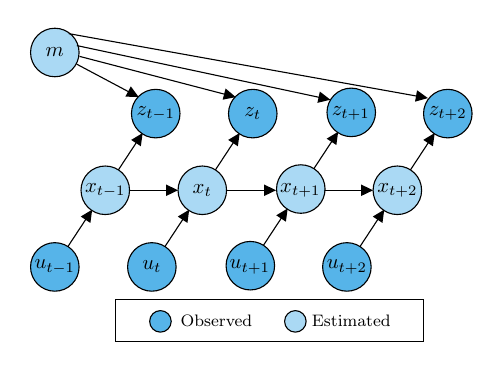
\begin{tikzpicture}[x=0.75pt,y=0.75pt,yscale=-0.65,xscale=0.65, every node/.style={scale=0.75}]
%uncomment if require: \path (0,208); %set diagram left start at 0, and has height of 208

%Shape: Ellipse [id:dp752950454176186] 
\draw  [fill=skyblue  ,fill opacity=0.5 ] (75.64,124.11) .. controls (75.64,114.18) and (83.69,106.13) .. (93.63,106.13) .. controls (103.56,106.13) and (111.61,114.18) .. (111.61,124.11) .. controls (111.61,134.04) and (103.56,142.1) .. (93.63,142.1) .. controls (83.69,142.1) and (75.64,134.04) .. (75.64,124.11) -- cycle ;
%Shape: Ellipse [id:dp19953500150518944] 
\draw  [fill=skyblue  ,fill opacity=0.5 ] (38.24,21.98) .. controls (38.24,12.05) and (46.29,4) .. (56.22,4) .. controls (66.15,4) and (74.21,12.05) .. (74.21,21.98) .. controls (74.21,31.91) and (66.15,39.96) .. (56.22,39.96) .. controls (46.29,39.96) and (38.24,31.91) .. (38.24,21.98) -- cycle ;
%Shape: Ellipse [id:dp3162640438661388] 
\draw  [fill=skyblue  ,fill opacity=1 ] (38.24,180.93) .. controls (38.24,171) and (46.29,162.95) .. (56.22,162.95) .. controls (66.15,162.95) and (74.21,171) .. (74.21,180.93) .. controls (74.21,190.87) and (66.15,198.92) .. (56.22,198.92) .. controls (46.29,198.92) and (38.24,190.87) .. (38.24,180.93) -- cycle ;
%Straight Lines [id:da6995903018861204] 
\draw    (65.93,165.83) -- (82.82,140.17) ;
\draw [shift={(83.92,138.5)}, rotate = 483.34] [fill={rgb, 255:red, 0; green, 0; blue, 0 }  ][line width=0.75]  [draw opacity=0] (8.93,-4.29) -- (0,0) -- (8.93,4.29) -- cycle    ;

%Shape: Ellipse [id:dp857819504517237] 
\draw  [fill=skyblue  ,fill opacity=1 ] (113.04,67.29) .. controls (113.04,57.36) and (121.1,49.31) .. (131.03,49.31) .. controls (140.96,49.31) and (149.01,57.36) .. (149.01,67.29) .. controls (149.01,77.22) and (140.96,85.27) .. (131.03,85.27) .. controls (121.1,85.27) and (113.04,77.22) .. (113.04,67.29) -- cycle ;
%Straight Lines [id:da21954766285916139] 
\draw    (103.33,109.01) -- (120.22,83.35) ;
\draw [shift={(121.32,81.68)}, rotate = 483.34] [fill={rgb, 255:red, 0; green, 0; blue, 0 }  ][line width=0.75]  [draw opacity=0] (8.93,-4.29) -- (0,0) -- (8.93,4.29) -- cycle    ;

%Shape: Circle [id:dp25504081320826777] 
\draw  [fill=skyblue  ,fill opacity=0.5 ] (147.57,124.11) .. controls (147.57,114.18) and (155.62,106.13) .. (165.55,106.13) .. controls (175.48,106.13) and (183.53,114.18) .. (183.53,124.11) .. controls (183.53,134.04) and (175.48,142.1) .. (165.55,142.1) .. controls (155.62,142.1) and (147.57,134.04) .. (147.57,124.11) -- cycle ;
%Shape: Ellipse [id:dp13620840701848025] 
\draw  [fill=skyblue  ,fill opacity=1 ] (110.17,180.93) .. controls (110.17,171) and (118.22,162.95) .. (128.15,162.95) .. controls (138.08,162.95) and (146.13,171) .. (146.13,180.93) .. controls (146.13,190.87) and (138.08,198.92) .. (128.15,198.92) .. controls (118.22,198.92) and (110.17,190.87) .. (110.17,180.93) -- cycle ;
%Straight Lines [id:da2834668811467105] 
\draw    (110.89,124.11) -- (145.57,124.11) ;
\draw [shift={(147.57,124.11)}, rotate = 180] [fill={rgb, 255:red, 0; green, 0; blue, 0 }  ][line width=0.75]  [draw opacity=0] (8.93,-4.29) -- (0,0) -- (8.93,4.29) -- cycle    ;

%Straight Lines [id:da81901241798572] 
\draw    (137.86,165.83) -- (154.74,140.17) ;
\draw [shift={(155.84,138.5)}, rotate = 483.34] [fill={rgb, 255:red, 0; green, 0; blue, 0 }  ][line width=0.75]  [draw opacity=0] (8.93,-4.29) -- (0,0) -- (8.93,4.29) -- cycle    ;

%Shape: Ellipse [id:dp07313197777173464] 
\draw  [fill=skyblue  ,fill opacity=1 ] (184.97,67.29) .. controls (184.97,57.36) and (193.02,49.31) .. (202.95,49.31) .. controls (212.88,49.31) and (220.93,57.36) .. (220.93,67.29) .. controls (220.93,77.22) and (212.88,85.27) .. (202.95,85.27) .. controls (193.02,85.27) and (184.97,77.22) .. (184.97,67.29) -- cycle ;
%Straight Lines [id:da1168703196833174] 
\draw    (175.26,109.01) -- (192.14,83.35) ;
\draw [shift={(193.24,81.68)}, rotate = 483.34] [fill={rgb, 255:red, 0; green, 0; blue, 0 }  ][line width=0.75]  [draw opacity=0] (8.93,-4.29) -- (0,0) -- (8.93,4.29) -- cycle    ;

%Straight Lines [id:da7739166562404441] 
\draw    (183.53,124.11) -- (218.21,124.11) ;
\draw [shift={(220.21,124.11)}, rotate = 180] [fill={rgb, 255:red, 0; green, 0; blue, 0 }  ][line width=0.75]  [draw opacity=0] (8.93,-4.29) -- (0,0) -- (8.93,4.29) -- cycle    ;

%Shape: Ellipse [id:dp2576096090133372] 
\draw  [fill=skyblue  ,fill opacity=0.5 ] (292.14,124.11) .. controls (292.14,114.18) and (300.19,106.13) .. (310.12,106.13) .. controls (320.05,106.13) and (328.1,114.18) .. (328.1,124.11) .. controls (328.1,134.04) and (320.05,142.1) .. (310.12,142.1) .. controls (300.19,142.1) and (292.14,134.04) .. (292.14,124.11) -- cycle ;
%Shape: Ellipse [id:dp3273402353013959] 
\draw  [fill=skyblue  ,fill opacity=1 ] (254.74,180.93) .. controls (254.74,171) and (262.79,162.95) .. (272.72,162.95) .. controls (282.65,162.95) and (290.7,171) .. (290.7,180.93) .. controls (290.7,190.87) and (282.65,198.92) .. (272.72,198.92) .. controls (262.79,198.92) and (254.74,190.87) .. (254.74,180.93) -- cycle ;
%Straight Lines [id:da41467285701714696] 
\draw    (255.46,124.11) -- (290.14,124.11) ;
\draw [shift={(292.14,124.11)}, rotate = 180] [fill={rgb, 255:red, 0; green, 0; blue, 0 }  ][line width=0.75]  [draw opacity=0] (8.93,-4.29) -- (0,0) -- (8.93,4.29) -- cycle    ;

%Straight Lines [id:da1202025526448216] 
\draw    (282.43,165.83) -- (299.31,140.17) ;
\draw [shift={(300.41,138.5)}, rotate = 483.34] [fill={rgb, 255:red, 0; green, 0; blue, 0 }  ][line width=0.75]  [draw opacity=0] (8.93,-4.29) -- (0,0) -- (8.93,4.29) -- cycle    ;

%Shape: Ellipse [id:dp9251751997354981] 
\draw  [fill=skyblue  ,fill opacity=1 ] (329.54,67.29) .. controls (329.54,57.36) and (337.59,49.31) .. (347.52,49.31) .. controls (357.45,49.31) and (365.5,57.36) .. (365.5,67.29) .. controls (365.5,77.22) and (357.45,85.27) .. (347.52,85.27) .. controls (337.59,85.27) and (329.54,77.22) .. (329.54,67.29) -- cycle ;
%Straight Lines [id:da9634878061709561] 
\draw    (319.83,109.01) -- (336.71,83.35) ;
\draw [shift={(337.81,81.68)}, rotate = 483.34] [fill={rgb, 255:red, 0; green, 0; blue, 0 }  ][line width=0.75]  [draw opacity=0] (8.93,-4.29) -- (0,0) -- (8.93,4.29) -- cycle    ;

%Straight Lines [id:da10960625166093363] 
\draw    (72.41,30.61) -- (116.67,54.13) ;
\draw [shift={(118.44,55.07)}, rotate = 207.98] [fill={rgb, 255:red, 0; green, 0; blue, 0 }  ][line width=0.75]  [draw opacity=0] (8.93,-4.29) -- (0,0) -- (8.93,4.29) -- cycle    ;

%Straight Lines [id:da0971567971199504] 
\draw    (74.56,24.86) -- (188.43,54.56) ;
\draw [shift={(190.36,55.07)}, rotate = 194.62] [fill={rgb, 255:red, 0; green, 0; blue, 0 }  ][line width=0.75]  [draw opacity=0] (8.93,-4.29) -- (0,0) -- (8.93,4.29) -- cycle    ;

%Straight Lines [id:da006621721555428728] 
\draw    (66.5,8) -- (330.81,55.43) ;
\draw [shift={(332.77,55.79)}, rotate = 190.17] [fill={rgb, 255:red, 0; green, 0; blue, 0 }  ][line width=0.75]  [draw opacity=0] (8.93,-4.29) -- (0,0) -- (8.93,4.29) -- cycle    ;


%Shape: Circle [id:dp258453978722042] 
\draw  [fill=skyblue  ,fill opacity=0.5 ] (220.57,123.2) .. controls (220.57,113.27) and (228.62,105.22) .. (238.55,105.22) .. controls (248.48,105.22) and (256.53,113.27) .. (256.53,123.2) .. controls (256.53,133.13) and (248.48,141.18) .. (238.55,141.18) .. controls (228.62,141.18) and (220.57,133.13) .. (220.57,123.2) -- cycle ;
%Shape: Ellipse [id:dp7767781831361724] 
\draw  [fill=skyblue  ,fill opacity=1 ] (183.17,180.02) .. controls (183.17,170.09) and (191.22,162.04) .. (201.15,162.04) .. controls (211.08,162.04) and (219.13,170.09) .. (219.13,180.02) .. controls (219.13,189.95) and (211.08,198) .. (201.15,198) .. controls (191.22,198) and (183.17,189.95) .. (183.17,180.02) -- cycle ;
%Straight Lines [id:da8933380774646036] 
\draw    (210.86,164.91) -- (227.74,139.25) ;
\draw [shift={(228.84,137.58)}, rotate = 483.34] [fill={rgb, 255:red, 0; green, 0; blue, 0 }  ][line width=0.75]  [draw opacity=0] (8.93,-4.29) -- (0,0) -- (8.93,4.29) -- cycle    ;

%Shape: Ellipse [id:dp922184729428642] 
\draw  [fill=skyblue  ,fill opacity=1 ] (257.97,66.38) .. controls (257.97,56.45) and (266.02,48.4) .. (275.95,48.4) .. controls (285.88,48.4) and (293.93,56.45) .. (293.93,66.38) .. controls (293.93,76.31) and (285.88,84.36) .. (275.95,84.36) .. controls (266.02,84.36) and (257.97,76.31) .. (257.97,66.38) -- cycle ;
%Straight Lines [id:da10273340205637205] 
\draw    (248.26,108.09) -- (265.14,82.43) ;
\draw [shift={(266.24,80.76)}, rotate = 483.34] [fill={rgb, 255:red, 0; green, 0; blue, 0 }  ][line width=0.75]  [draw opacity=0] (8.93,-4.29) -- (0,0) -- (8.93,4.29) -- cycle    ;

%Straight Lines [id:da8888451886953346] 
\draw    (72.56,16.86) -- (258.54,56.58) ;
\draw [shift={(260.5,57)}, rotate = 192.06] [fill={rgb, 255:red, 0; green, 0; blue, 0 }  ][line width=0.75]  [draw opacity=0] (8.93,-4.29) -- (0,0) -- (8.93,4.29) -- cycle    ;


%Shape: Rectangle [id:dp5382524014123531] 
\draw   (101.5,205) -- (329.5,205) -- (329.5,236) -- (101.5,236) -- cycle ;
%Shape: Ellipse [id:dp15178603313610284] 
\draw  [fill=skyblue  ,fill opacity=1 ] (126.54,221.29) .. controls (126.54,216.89) and (130.11,213.31) .. (134.52,213.31) .. controls (138.93,213.31) and (142.5,216.89) .. (142.5,221.29) .. controls (142.5,225.7) and (138.93,229.27) .. (134.52,229.27) .. controls (130.11,229.27) and (126.54,225.7) .. (126.54,221.29) -- cycle ;
%Shape: Ellipse [id:dp18259132951806] 
\draw  [fill=skyblue  ,fill opacity=0.5 ] (226.54,221.29) .. controls (226.54,216.89) and (230.11,213.31) .. (234.52,213.31) .. controls (238.93,213.31) and (242.5,216.89) .. (242.5,221.29) .. controls (242.5,225.7) and (238.93,229.27) .. (234.52,229.27) .. controls (230.11,229.27) and (226.54,225.7) .. (226.54,221.29) -- cycle ;

% Text Node
\draw (93.63,124.11) node   {$\boldsymbol{x}_{t-1}$};
% Text Node
\draw (56.22,21.98) node   {$\boldsymbol{m}$};
% Text Node
\draw (56.22,180.93) node   {$\boldsymbol{u}_{t-1}$};
% Text Node
\draw (131.03,67.29) node   {$\boldsymbol{z}_{t-1}$};
% Text Node
\draw (165.55,124.11) node   {$\boldsymbol{x}_{t}$};
% Text Node
\draw (128.15,180.93) node   {$\boldsymbol{u}_{t}$};
% Text Node
\draw (202.95,67.29) node   {$\boldsymbol{z}_{t}$};
% Text Node
\draw (238.19,124.11) node   {$\boldsymbol{x}_{t+1}$};
% Text Node
\draw (200.79,180.93) node   {$\boldsymbol{u}_{t+1}$};
% Text Node
\draw (275.59,67.29) node   {$\boldsymbol{z}_{t+1}$};
% Text Node
\draw (310.12,124.11) node   {$\boldsymbol{x}_{t+2}$};
% Text Node
\draw (272.72,180.93) node   {$\boldsymbol{u}_{t+2}$};
% Text Node
\draw (347.52,67.29) node   {$\boldsymbol{z}_{t+2}$};
% Text Node
\draw (176,221) node  [align=left] {{\footnotesize Observed}};
% Text Node
\draw (276,221) node  [align=left] {{\footnotesize Estimated}};


\end{tikzpicture}

					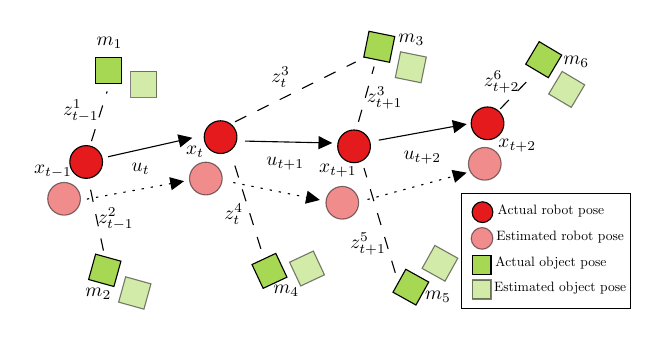
\begin{tikzpicture}[x=0.70pt,y=0.70pt,yscale=-0.60,xscale=0.60, every node/.style={scale=0.70}]
%uncomment if require: \path (0,258); %set diagram left start at 0, and has height of 258

%Shape: Ellipse [id:dp7434301091862943] 
\draw  [color=black  ,draw opacity=0.5 ][fill=red  ,fill opacity=0.5 ] (6.44,153.49) .. controls (6.44,145.72) and (12.74,139.42) .. (20.52,139.42) .. controls (28.29,139.42) and (34.6,145.72) .. (34.6,153.49) .. controls (34.6,161.27) and (28.29,167.57) .. (20.52,167.57) .. controls (12.74,167.57) and (6.44,161.27) .. (6.44,153.49) -- cycle ;
%Shape: Rectangle [id:dp6808133197576726] 
\draw  [color=black  ,draw opacity=1 ][fill=green  ,fill opacity=1 ] (47.63,31.7) -- (70.24,31.7) -- (70.24,54.31) -- (47.63,54.31) -- cycle ;
%Shape: Ellipse [id:dp13056961037551362] 
\draw  [color=black  ,draw opacity=0.5 ][fill=red  ,fill opacity=0.5 ] (128.41,136.07) .. controls (128.41,128.29) and (134.72,121.99) .. (142.49,121.99) .. controls (150.27,121.99) and (156.57,128.29) .. (156.57,136.07) .. controls (156.57,143.84) and (150.27,150.15) .. (142.49,150.15) .. controls (134.72,150.15) and (128.41,143.84) .. (128.41,136.07) -- cycle ;
%Shape: Ellipse [id:dp9996445403573203] 
\draw  [color=black  ,draw opacity=0.5 ][fill=red  ,fill opacity=0.5 ] (245.81,156.91) .. controls (245.81,149.13) and (252.11,142.83) .. (259.89,142.83) .. controls (267.66,142.83) and (273.97,149.13) .. (273.97,156.91) .. controls (273.97,164.68) and (267.66,170.99) .. (259.89,170.99) .. controls (252.11,170.99) and (245.81,164.68) .. (245.81,156.91) -- cycle ;
%Shape: Ellipse [id:dp1885221377208316] 
\draw  [color=black  ,draw opacity=0.5 ][fill=red  ,fill opacity=0.5 ] (368.4,123.4) .. controls (368.4,115.62) and (374.7,109.32) .. (382.48,109.32) .. controls (390.25,109.32) and (396.55,115.62) .. (396.55,123.4) .. controls (396.55,131.17) and (390.25,137.47) .. (382.48,137.47) .. controls (374.7,137.47) and (368.4,131.17) .. (368.4,123.4) -- cycle ;
%Shape: Ellipse [id:dp5392362763171864] 
\draw  [fill=red  ,fill opacity=1 ] (25.45,121.81) .. controls (25.45,114.04) and (31.75,107.73) .. (39.53,107.73) .. controls (47.3,107.73) and (53.61,114.04) .. (53.61,121.81) .. controls (53.61,129.59) and (47.3,135.89) .. (39.53,135.89) .. controls (31.75,135.89) and (25.45,129.59) .. (25.45,121.81) -- cycle ;
%Shape: Ellipse [id:dp9130435739184759] 
\draw  [fill=red  ,fill opacity=1 ] (141.09,100.43) .. controls (141.09,92.65) and (147.39,86.35) .. (155.16,86.35) .. controls (162.94,86.35) and (169.24,92.65) .. (169.24,100.43) .. controls (169.24,108.2) and (162.94,114.51) .. (155.16,114.51) .. controls (147.39,114.51) and (141.09,108.2) .. (141.09,100.43) -- cycle ;
%Shape: Ellipse [id:dp11001638797843405] 
\draw  [fill=red  ,fill opacity=1 ] (255.93,108.35) .. controls (255.93,100.57) and (262.23,94.27) .. (270.01,94.27) .. controls (277.78,94.27) and (284.09,100.57) .. (284.09,108.35) .. controls (284.09,116.12) and (277.78,122.43) .. (270.01,122.43) .. controls (262.23,122.43) and (255.93,116.12) .. (255.93,108.35) -- cycle ;
%Shape: Ellipse [id:dp21523771226438004] 
\draw  [fill=red  ,fill opacity=1 ] (370.77,88.55) .. controls (370.77,80.77) and (377.08,74.47) .. (384.85,74.47) .. controls (392.63,74.47) and (398.93,80.77) .. (398.93,88.55) .. controls (398.93,96.32) and (392.63,102.63) .. (384.85,102.63) .. controls (377.08,102.63) and (370.77,96.32) .. (370.77,88.55) -- cycle ;
%Shape: Rectangle [id:dp39352313397759164] 
\draw  [color=black  ,draw opacity=0.5 ][fill=green  ,fill opacity=0.5 ] (77.72,43.58) -- (100.34,43.58) -- (100.34,66.19) -- (77.72,66.19) -- cycle ;
%Shape: Rectangle [id:dp10940816352865923] 
\draw  [color=black  ,draw opacity=1 ][fill=green  ,fill opacity=1 ] (47.64,201.12) -- (69.44,207.16) -- (63.4,228.95) -- (41.61,222.91) -- cycle ;
%Shape: Rectangle [id:dp45450106813081703] 
\draw  [color=black  ,draw opacity=0.5 ][fill=green  ,fill opacity=0.5 ] (73.48,220.6) -- (95.27,226.64) -- (89.23,248.43) -- (67.44,242.4) -- cycle ;
%Shape: Rectangle [id:dp2630909080760764] 
\draw  [color=black  ,draw opacity=1 ][fill=green  ,fill opacity=1 ] (182.2,210.05) -- (202.67,200.45) -- (212.27,220.93) -- (191.79,230.52) -- cycle ;
%Shape: Rectangle [id:dp7021199786756188] 
\draw  [color=black  ,draw opacity=0.5 ][fill=green  ,fill opacity=0.5 ] (214.49,208.03) -- (234.97,198.44) -- (244.56,218.91) -- (224.09,228.51) -- cycle ;
%Shape: Rectangle [id:dp8406498517381461] 
\draw  [color=black  ,draw opacity=1 ][fill=green  ,fill opacity=1 ] (282.86,9.37) -- (305.02,13.87) -- (300.52,36.03) -- (278.36,31.53) -- cycle ;
%Shape: Rectangle [id:dp5992753478320311] 
\draw  [color=black  ,draw opacity=0.5 ][fill=green  ,fill opacity=0.5 ] (309.99,27.01) -- (332.15,31.51) -- (327.65,53.67) -- (305.49,49.17) -- cycle ;
%Shape: Rectangle [id:dp48388398423368595] 
\draw  [color=black  ,draw opacity=0.5 ][fill=green  ,fill opacity=0.5 ] (359.28,204.6) -- (348.28,224.35) -- (328.52,213.35) -- (339.52,193.6) -- cycle ;
%Shape: Rectangle [id:dp44335535839655893] 
\draw  [color=black  ,draw opacity=1 ][fill=green  ,fill opacity=1 ] (334.26,225.11) -- (323.26,244.87) -- (303.5,233.87) -- (314.5,214.11) -- cycle ;
%Shape: Rectangle [id:dp2110614236699101] 
\draw  [color=black  ,draw opacity=1 ][fill=green  ,fill opacity=1 ] (429.25,18.27) -- (448.67,29.84) -- (437.11,49.27) -- (417.68,37.7) -- cycle ;
%Shape: Rectangle [id:dp734525975812425] 
\draw  [color=black  ,draw opacity=0.5 ][fill=green  ,fill opacity=0.5 ] (449.03,43.87) -- (468.46,55.44) -- (456.89,74.87) -- (437.46,63.3) -- cycle ;
%Straight Lines [id:da8771117550774294] 
\draw    (58.36,117.3) -- (126.9,101.9) ;
\draw [shift={(128.85,101.46)}, rotate = 527.3299999999999] [fill={rgb, 255:red, 0; green, 0; blue, 0 }  ][line width=0.75]    (8.93,-4.29) -- (0,0) -- (8.93,4.29) -- cycle    ;

%Straight Lines [id:da7204140282863669] 
\draw  [dash pattern={on 0.84pt off 2.51pt}]  (40.14,153.74) -- (119.75,139.05) ;
\draw [shift={(121.72,138.69)}, rotate = 529.55] [fill={rgb, 255:red, 0; green, 0; blue, 0 }  ][line width=0.75]    (8.93,-4.29) -- (0,0) -- (8.93,4.29) -- cycle    ;

%Straight Lines [id:da8591492656423307] 
\draw    (176.37,103.84) -- (247.24,105.38) ;
\draw [shift={(249.24,105.42)}, rotate = 181.25] [fill={rgb, 255:red, 0; green, 0; blue, 0 }  ][line width=0.75]    (8.93,-4.29) -- (0,0) -- (8.93,4.29) -- cycle    ;

%Straight Lines [id:da09058967319467015] 
\draw  [dash pattern={on 0.84pt off 2.51pt}]  (166.07,139.48) -- (236.59,153.69) ;
\draw [shift={(238.55,154.08)}, rotate = 191.39] [fill={rgb, 255:red, 0; green, 0; blue, 0 }  ][line width=0.75]    (8.93,-4.29) -- (0,0) -- (8.93,4.29) -- cycle    ;

%Straight Lines [id:da6287850967405952] 
\draw    (291.21,103.05) -- (362.91,89.94) ;
\draw [shift={(364.87,89.58)}, rotate = 529.64] [fill={rgb, 255:red, 0; green, 0; blue, 0 }  ][line width=0.75]    (8.93,-4.29) -- (0,0) -- (8.93,4.29) -- cycle    ;

%Straight Lines [id:da39601612623948923] 
\draw  [dash pattern={on 0.84pt off 2.51pt}]  (281.55,154.08) -- (362.94,132.08) ;
\draw [shift={(364.87,131.56)}, rotate = 524.87] [fill={rgb, 255:red, 0; green, 0; blue, 0 }  ][line width=0.75]    (8.93,-4.29) -- (0,0) -- (8.93,4.29) -- cycle    ;

%Straight Lines [id:da14218951162996163] 
\draw  [dash pattern={on 4.5pt off 4.5pt}]  (44.1,103.84) -- (57.57,61.07) ;


%Straight Lines [id:da5099949144358528] 
\draw  [dash pattern={on 4.5pt off 4.5pt}]  (54.4,198.09) -- (42.52,141.86) ;


%Straight Lines [id:da8152861145371411] 
\draw  [dash pattern={on 4.5pt off 4.5pt}]  (167.66,87.21) -- (271.41,35.73) ;


%Straight Lines [id:da6504983020328421] 
\draw  [dash pattern={on 4.5pt off 4.5pt}]  (273.79,87.21) -- (287.25,39.69) ;


%Straight Lines [id:da09932466850869759] 
\draw  [dash pattern={on 4.5pt off 4.5pt}]  (189.83,196.51) -- (166.07,120.47) ;


%Straight Lines [id:da5252262954209137] 
\draw  [dash pattern={on 4.5pt off 4.5pt}]  (305.47,217.1) -- (278.55,127.08) ;


%Straight Lines [id:da11641625781770915] 
\draw  [dash pattern={on 4.5pt off 4.5pt}]  (395.76,76.12) -- (423.48,47.61) ;


%Shape: Rectangle [id:dp779804859980624] 
\draw   (362.5,148.99) -- (507.55,148.99) -- (507.55,247.99) -- (362.5,247.99) -- cycle ;
%Shape: Circle [id:dp9912886474851581] 
\draw  [fill=red  ,fill opacity=1 ] (371.57,164.98) .. controls (371.57,160.05) and (375.56,156.05) .. (380.5,156.05) .. controls (385.43,156.05) and (389.43,160.05) .. (389.43,164.98) .. controls (389.43,169.91) and (385.43,173.91) .. (380.5,173.91) .. controls (375.56,173.91) and (371.57,169.91) .. (371.57,164.98) -- cycle ;
%Shape: Ellipse [id:dp633215489310963] 
\draw  [color=black  ,draw opacity=0.5 ][fill=red  ,fill opacity=0.5 ] (370.77,187.55) .. controls (370.77,182.4) and (374.95,178.22) .. (380.1,178.22) .. controls (385.25,178.22) and (389.43,182.4) .. (389.43,187.55) .. controls (389.43,192.7) and (385.25,196.88) .. (380.1,196.88) .. controls (374.95,196.88) and (370.77,192.7) .. (370.77,187.55) -- cycle ;
%Shape: Square [id:dp9486488989130497] 
\draw  [color=black  ,draw opacity=1 ][fill=green  ,fill opacity=1 ] (371.57,201.99) -- (387.84,201.99) -- (387.84,218.26) -- (371.57,218.26) -- cycle ;
%Shape: Square [id:dp13355255501454244] 
\draw  [color=black  ,draw opacity=0.5 ][fill=green  ,fill opacity=0.5 ] (371.57,223.37) -- (387.84,223.37) -- (387.84,239.65) -- (371.57,239.65) -- cycle ;

% Text Node
\draw (10.98,129.95) node   {$\boldsymbol{x}_{t-1}$};
% Text Node
\draw (133.17,113.11) node   {$\boldsymbol{x}_{t}$};
% Text Node
\draw (256.02,129.53) node   {$\boldsymbol{x}_{t+1}$};
% Text Node
\draw (410.38,107.73) node   {$\boldsymbol{x}_{t+2}$};
% Text Node
\draw (86.44,127.53) node   {$\boldsymbol{u}_{t}$};
% Text Node
\draw (210.78,123.57) node   {$\boldsymbol{u}_{t+1}$};
% Text Node
\draw (328.8,118.03) node   {$\boldsymbol{u}_{t+2}$};
% Text Node
\draw (34.95,77.64) node   {$\boldsymbol{z}^{1}_{t-1}$};
% Text Node
\draw (65.05,171.1) node   {$\boldsymbol{z}^{2}_{t-1}$};
% Text Node
\draw (206.82,49.12) node   {$\boldsymbol{z}^{3}_{t}$};
% Text Node
\draw (166.43,166.34) node   {$\boldsymbol{z}^{4}_{t}$};
% Text Node
\draw (296.32,66.55) node   {$\boldsymbol{z}^{3}_{t+1}$};
% Text Node
\draw (282.07,192.48) node   {$\boldsymbol{z}^{5}_{t+1}$};
% Text Node
\draw (396.91,53.08) node   {$\boldsymbol{z}^{6}_{t+2}$};
% Text Node
\draw (59.51,19.03) node   {$\boldsymbol{m}_{1}$};
% Text Node
\draw (50,235.25) node   {$\boldsymbol{m}_{2}$};
% Text Node
\draw (319.29,16.65) node   {$\boldsymbol{m}_{3}$};
% Text Node
\draw (211.58,232.87) node   {$\boldsymbol{m}_{4}$};
% Text Node
\draw (342.26,237.63) node   {$\boldsymbol{m}_{5}$};
% Text Node
\draw (461.07,35.66) node   {$\boldsymbol{m}_{6}$};
% Text Node
\draw (439.34,163.97) node [scale=0.7] [align=left] {Actual robot pose};
% Text Node
\draw (447.34,186.14) node [scale=0.7] [align=left] {Estimated robot pose};
% Text Node
\draw (439.34,209.11) node [scale=0.7] [align=left] {Actual object pose};
% Text Node
\draw (447.34,230.5) node [scale=0.7] [align=left] {Estimated object pose};

\end{tikzpicture}
					\caption{\centering \footnotesize Example of the SLAM problem (DURRANT-WHYTE; BAILEY, 2006)}.	
				\end{figure}
			\end{center}
		%\end{column}
	%\end{columns}    
}

\frame{
	\frametitle{Loop Closure Detection}
	\begin{columns}
		\begin{column}{0.5\textwidth}
			\begin{itemize}
				\justifying
				\item Estimation errors accumulated during movement increase the pose uncertainty and drifting;
				\item Recognize previously visited places, reducing uncertainty and updating the map.
			\end{itemize}
		\end{column}
		%falar da imagem
		\begin{column}{0.5\textwidth}  %%<--- here
			\begin{center}
				\begin{figure}
					\label{figure:fig3}
					\includegraphics[scale=0.35, height=80pt, width=110pt]{maperrors2.pdf}
					
					\caption{\centering \footnotesize Map built using only odometry (CADENA et al., 2016).}
				\end{figure}
			\end{center}
		\end{column}
	\end{columns}    
}

\frame{
	\frametitle{How to detect loop closures?}
	\begin{itemize}
		\justifying
		\item Correspondence search using appearance signatures from places visited during the trajectory;
		\item Signatures can be built using shape, color and other data available from sensors:
		\begin{itemize}
			\justifying
			\item Several visual-based methods\footnote[frame]{\tiny (CUMMINS; NEWMAN, 2008; MILFORD; WYETH, 2012; LOWRY et al., 2016)} for cameras developed over the past years;
			\item 3D LIDAR-based methods are considered less mature\footnote[frame]{\tiny (HE; WANG; ZHANG, 2016; DUB{\'E} et al., 2017)}.		
		\end{itemize}
	\end{itemize}
}
%%PENSAR EM COMO APRESENTAR A CONEXÃO DO SLIDE ACIMA PARA O DE BAIXO
\frame{
	\frametitle{Point Cloud Descriptors}
	\begin{itemize}
		\justifying
		\item Typically, loop closure detection with 3D LIDARs employ point cloud matching approaches\footnote[frame]{\tiny (BOSSE; ZLOT, 2013; CIESLEWSKI et al., 2016; HE; WANG; ZHANG, 2016)} using feature descriptors:
		\begin{itemize}
			\justifying
			\item Global descriptors represent the entire cloud geometry into a single descriptor;
			\item Local descriptors compute the characteristics around multiple keypoints:
			\begin{itemize}
				\justifying
				\item Quality and performance issues with keypoint detection techniques\footnote[frame]{\tiny (DUBÉ et al., 2017)}.	
			\end{itemize}					
		\end{itemize}
	\end{itemize}
}

\frame{
	\frametitle{Multiview 2D Projection (M2DP)}
	\begin{itemize}
		\justifying
		\item Recently, the M2DP\footnote[frame]{\tiny (HE; WANG; ZHANG, 2016)} descriptor presented significant results when applied to loop closure detection:
		\begin{itemize}
			\justifying  
			\item Outperforms other descriptors, such as SHOT\footnote[frame]{\tiny (TOMBARI; SALTI; STEFANO, 2011)}'s global variant;			
			\item Avoids using normals, which can be costly to estimate for large clouds;
			\item Spatial density distributions are computed from multiple 2D projections of a point cloud;
		\end{itemize}
		\item We noticed that it could be extended to compute additional information from each projection.
		%\item Detecting loop closures comes down to finding the most similar descriptors, using the $L2$ norm.		
	\end{itemize}
}

\section{Proposal}
\frame{
	\frametitle{Combining Color and Shape}
	\begin{columns}
		\begin{column}{0.5\textwidth}
			\begin{itemize}
				\justifying
				\item Alongside 3D spatial data, color can provide more descriptive scenes:
				\begin{itemize}
					\justifying
					\item Object recognition works\footnote[frame]{\tiny (TOMBARI; SALTI; STEFANO, 2011; FENG; LIU; LIAO, 2015; LOGOGLU; KALKAN; TEMIZEL, 2016)} report increase in descriptiveness;
					\item Insufficiently investigated approach for loop closure detection.
				\end{itemize}
				%\item 3D spatial data can provide more descriptive scenes than only 2D images;
				%\item Sensor availability in recent bechmark platforms\footnote[frame]{\tiny (PANDEY; MCBRIDE; EUSTICE, 2011; GEIGER; LENZ; URTASUN, 2012)}.   
			\end{itemize}
		\end{column}
		\begin{column}{0.5\textwidth}  %%<--- here
			\begin{center}
				\begin{figure}[h!]
					\centering
					\includegraphics[scale=0.35, height=50pt, width=\textwidth]{2_419lidar2.png}
					
					\includegraphics[scale=0.35, height=50pt, width=\textwidth]{3_419lidarcamera2.png}
					
					\caption{\centering \footnotesize Colored point cloud generated using LIDAR and camera.}
					\label{fig:pointclouds}
				\end{figure}
			\end{center}
		\end{column}
	\end{columns}  
}

\frame{
	\frametitle{Our Approach}
	\centering
	\large \textbf{Color M2DP (c-M2DP)}
	\begin{itemize}
		\justifying
		\item A global descriptor comprising of color and shape data computed from the point cloud;
		\item An improved loop closure detection, using the c-M2DP descriptor on point cloud sequences generated through camera-LIDAR fusion, or stereo depth estimation.
		%falar da densidade
	\end{itemize}
}

\section{Related Work}
\frame{
	\frametitle{Loop Closure Detection using Point Cloud Descriptors}
	\begin{itemize}
		\justifying
		%\item Cylindrical support with radial, azimuthal and vertical splits;
		\item Both avoid using normals, measuring point distributions from the point clouds; %from sparse (NBLD) or dense, but downsampled (3D Gestalt) clouds;
		\item However, both are local descriptors, and compute only shape data from the cloud.
		%\item Local, shape-only descriptors for dense, but downsampled (3D Gestalt), or sparse (NBLD) point clouds; 
		%focar que não foram comparados por serem locais
	\end{itemize}
	\begin{columns}
	\begin{column}{0.5\textwidth}		
		\begin{figure}
			\vspace{-0.5em}
			\label{figure:gestalt}
			\includegraphics[height=80pt, width=0.8\textwidth]{gestalt.png}
			\caption{\centering \footnotesize 3D Gestalt (BOSSE; ZLOT, 2013).}
		\end{figure}
	\end{column}	
	\begin{column}{0.5\textwidth}  %%<--- here
		\begin{center}
		\begin{figure}
			\label{figure:nbld}
			\includegraphics[height=80pt, width=0.8\textwidth]{nbld.png}
			\caption{\centering \footnotesize NBLD (CIESLEWSKI et al., 2016).}
		\end{figure}
		\end{center}
	\end{column}
	\end{columns}	
}

\frame{
	\frametitle{Color and Shape Point Cloud Descriptors}	
	\begin{itemize}
		\justifying
		\item Local descriptors designed for object recognition applications:
		\begin{itemize}
			\justifying
			\item Histograms of normals and color characteristics are computed from a local support split in concentric spheres;		
		\end{itemize}		
		\item Additionally, CSHOT have a global variant that uses the whole cloud as support.
		%\item Local, spherical support with radial splits around keypoints;
		%\item Histograms of angular relations between surface normals, and color intensities;
	\end{itemize}
	\begin{columns}
	\begin{column}{0.5\textwidth}		
	\begin{figure}
		\label{figure:cshot}
		\includegraphics[height=80pt, width=\textwidth]{cshot.png}
		\caption{\centering \footnotesize CSHOT (TOMBARI; SALTI; STEFANO, 2011).}
	\end{figure}
	\end{column}	
	\begin{column}{0.5\textwidth}  %%<--- here
	\begin{center}
	\begin{figure}
		\vspace{-3em}
		\label{figure:cospair}
		\includegraphics[height=100pt, width=\textwidth]{cospair.png}
		\caption{\centering \footnotesize CoSPAIR (LOGOGLU; KALKAN; TEMIZEL, 2016).}
	\end{figure}
	\end{center}
	\end{column}
	\end{columns}   
}

\section{c-M2DP}
\frame{
	\frametitle{Extending M2DP}
	\begin{itemize}
		\justifying
		\item Our proposal takes advantage of M2DP's existing structure:
		\begin{itemize}
			\justifying
			\item Reference frame, shape signatures, and dimensionality reduction steps remains unchanged;
			\item Color signatures are computed alongside shape, from the multiple 2D projections;
			\item Increased length of signature matrix and descriptor vector.
		\end{itemize}			
	\end{itemize}
}

\frame{
	\frametitle{Reference Frame}
	\begin{itemize}
		\justifying
		\item Point cloud $\boldsymbol{P}$ centroid is computed and used as the reference frame origin;
		\item PCA is performed on $\boldsymbol{P}$, with the 1st and 2nd PCs defined as the $x$-axis and $y$-axis, respectively.
	\end{itemize}
}

\frame{
	\frametitle{Multiple 2D Projections}
	\begin{columns}
	\begin{column}{0.5\textwidth}
		\begin{itemize}
			\justifying
			\item Distinct 2D planes are generated by varying $[\theta, \phi]$;
			\item  $\boldsymbol{P}$ is projected onto each 2D plane, in order to compute shape and color signatures from each 2D projection.
		\end{itemize}
	\end{column}
	\begin{column}{0.5\textwidth}  %%<--- here
		\begin{center}
		\begin{figure}[h!]
			\centering
			\vspace{-1em}
			\begin{tikzpicture}[x=0.75pt,y=0.75pt,yscale=-0.6,xscale=0.6]
%uncomment if require: \path (0,300); %set diagram left start at 0, and has height of 300

%Image [id:dp09254054009459467] 
\draw (94.52,11.18) node  {\includegraphics[width=79pt,height=70pt]{pointcloud.pdf}};
%Image [id:dp26150135761132864] 
\draw (15.52,166.18) node  {\includegraphics[width=79pt,height=70pt]{projection1.pdf}};
%Image [id:dp6062331233282552] 
\draw (192.52,166.18) node  {\includegraphics[width=79pt,height=70pt]{projection2.pdf}};
%Down Arrow [id:dp6057459970471565] 
\draw   (77,99.95) -- (84.51,99.95) -- (84.51,89.37) -- (115.52,89.37) -- (115.52,99.95) -- (120.03,99.95) -- (99.02,110) -- cycle ;

% Text Node
\draw (99.75,168.41) node  [align=left, scale=1.2] {\dots};


\end{tikzpicture}

			\vspace{-2em}
			\caption{\centering \footnotesize Projecting $\boldsymbol{P}$ on multiple 2D planes.}
			\label{fig:multiple-projections}	
		\end{figure}
		\end{center}
	\end{column}
	\end{columns}	
}

\frame{
	\frametitle{Shape Signature}
	\begin{columns}
	\begin{column}{0.5\textwidth}
		\begin{itemize}
			\justifying
			\item Each plane is split into $l$ concentric circles;
			\item Each concentric circle is divided in $h$ shape bins, indexed by the $x$-axis; 
			\item Shape signature $\boldsymbol{s}^X$ is computed by counting the points within each bin.
		\end{itemize}
	\end{column}
	\begin{column}{0.5\textwidth}  %%<--- here
		\begin{center}
		\begin{figure}[h!]
			\centering
			\vspace{0.7cm}
			%\includegraphics[height=7cm]{shapesignature2.pdf}
			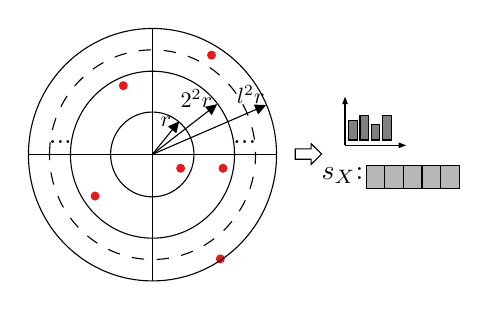
\begin{tikzpicture}[x=0.75pt,y=0.75pt,yscale=-0.6,xscale=0.6]
%uncomment if require: \path (0,388); %set diagram left start at 0, and has height of 388

%Shape: Ellipse [id:dp7382617193591512] 
\draw   (78.77,111.59) .. controls (78.77,92.78) and (93.76,77.53) .. (112.24,77.53) .. controls (130.73,77.53) and (145.71,92.78) .. (145.71,111.59) .. controls (145.71,130.4) and (130.73,145.64) .. (112.24,145.64) .. controls (93.76,145.64) and (78.77,130.4) .. (78.77,111.59) -- cycle ;
%Shape: Ellipse [id:dp25517697407182616] 
\draw   (46.54,111.77) .. controls (46.54,74.75) and (76.03,44.74) .. (112.42,44.74) .. controls (148.8,44.74) and (178.3,74.75) .. (178.3,111.77) .. controls (178.3,148.79) and (148.8,178.8) .. (112.42,178.8) .. controls (76.03,178.8) and (46.54,148.79) .. (46.54,111.77) -- cycle ;
%Shape: Ellipse [id:dp3459858941325883] 
\draw  [dash pattern={on 4.5pt off 4.5pt}] (29.7,111.77) .. controls (29.7,65.29) and (66.73,27.6) .. (112.42,27.6) .. controls (158.1,27.6) and (195.14,65.29) .. (195.14,111.77) .. controls (195.14,158.25) and (158.1,195.94) .. (112.42,195.94) .. controls (66.73,195.94) and (29.7,158.25) .. (29.7,111.77) -- cycle ;
%Shape: Ellipse [id:dp06494650200316232] 
\draw  [color={rgb, 255:red, 255; green, 0; blue, 0 }  ,draw opacity=1 ][fill={rgb, 255:red, 255; green, 0; blue, 0 }  ,fill opacity=1 ] (131.9,122.66) .. controls (131.9,120.92) and (133.29,119.51) .. (135,119.51) .. controls (136.72,119.51) and (138.11,120.92) .. (138.11,122.66) .. controls (138.11,124.41) and (136.72,125.82) .. (135,125.82) .. controls (133.29,125.82) and (131.9,124.41) .. (131.9,122.66) -- cycle ;
%Shape: Ellipse [id:dp0022695334650385535] 
\draw  [color={rgb, 255:red, 255; green, 0; blue, 0 }  ,draw opacity=1 ][fill={rgb, 255:red, 255; green, 0; blue, 0 }  ,fill opacity=1 ] (165.9,122.66) .. controls (165.9,120.92) and (167.29,119.51) .. (169.01,119.51) .. controls (170.72,119.51) and (172.11,120.92) .. (172.11,122.66) .. controls (172.11,124.41) and (170.72,125.82) .. (169.01,125.82) .. controls (167.29,125.82) and (165.9,124.41) .. (165.9,122.66) -- cycle ;
%Shape: Ellipse [id:dp9477076352826888] 
\draw  [color={rgb, 255:red, 255; green, 0; blue, 0 }  ,draw opacity=1 ][fill={rgb, 255:red, 255; green, 0; blue, 0 }  ,fill opacity=1 ] (85.85,56.36) .. controls (85.85,54.61) and (87.24,53.2) .. (88.96,53.2) .. controls (90.67,53.2) and (92.06,54.61) .. (92.06,56.36) .. controls (92.06,58.1) and (90.67,59.51) .. (88.96,59.51) .. controls (87.24,59.51) and (85.85,58.1) .. (85.85,56.36) -- cycle ;
%Shape: Ellipse [id:dp34247701706686684] 
\draw  [color={rgb, 255:red, 255; green, 0; blue, 0 }  ,draw opacity=1 ][fill={rgb, 255:red, 255; green, 0; blue, 0 }  ,fill opacity=1 ] (156.69,31.85) .. controls (156.69,30.11) and (158.08,28.69) .. (159.8,28.69) .. controls (161.51,28.69) and (162.9,30.11) .. (162.9,31.85) .. controls (162.9,33.59) and (161.51,35.01) .. (159.8,35.01) .. controls (158.08,35.01) and (156.69,33.59) .. (156.69,31.85) -- cycle ;
%Shape: Ellipse [id:dp5637425041894341] 
\draw  [color={rgb, 255:red, 255; green, 0; blue, 0 }  ,draw opacity=1 ][fill={rgb, 255:red, 255; green, 0; blue, 0 }  ,fill opacity=1 ] (63.19,145.01) .. controls (63.19,143.26) and (64.58,141.85) .. (66.29,141.85) .. controls (68.01,141.85) and (69.4,143.26) .. (69.4,145.01) .. controls (69.4,146.75) and (68.01,148.17) .. (66.29,148.17) .. controls (64.58,148.17) and (63.19,146.75) .. (63.19,145.01) -- cycle ;
%Shape: Ellipse [id:dp3859458151744748] 
\draw  [color={rgb, 255:red, 255; green, 0; blue, 0 }  ,draw opacity=1 ][fill={rgb, 255:red, 255; green, 0; blue, 0 }  ,fill opacity=1 ] (163.78,195.46) .. controls (163.78,193.72) and (165.17,192.3) .. (166.88,192.3) .. controls (168.6,192.3) and (169.99,193.72) .. (169.99,195.46) .. controls (169.99,197.21) and (168.6,198.62) .. (166.88,198.62) .. controls (165.17,198.62) and (163.78,197.21) .. (163.78,195.46) -- cycle ;
%Straight Lines [id:da9093409121292956] 
\draw    (112.24,10.23) -- (112.24,212.94) ;


%Straight Lines [id:da6639286505692693] 
\draw    (12.63,111.59) -- (211.86,111.59) ;


%Straight Lines [id:da5044264629099462] 
\draw    (112.24,111.59) -- (132.58,86.46) ;
\draw [shift={(133.84,84.91)}, rotate = 488.99] [fill={rgb, 255:red, 0; green, 0; blue, 0 }  ][line width=0.75]  [draw opacity=0] (8.93,-4.29) -- (0,0) -- (8.93,4.29) -- cycle    ;

%Straight Lines [id:da8524918674228583] 
\draw    (112.24,111.59) -- (162.79,72.44) ;
\draw [shift={(164.38,71.21)}, rotate = 502.25] [fill={rgb, 255:red, 0; green, 0; blue, 0 }  ][line width=0.75]  [draw opacity=0] (8.93,-4.29) -- (0,0) -- (8.93,4.29) -- cycle    ;

%Straight Lines [id:da5923697154582754] 
\draw    (112.24,111.59) -- (201.87,72.73) ;
\draw [shift={(203.71,71.94)}, rotate = 516.56] [fill={rgb, 255:red, 0; green, 0; blue, 0 }  ][line width=0.75]  [draw opacity=0] (8.93,-4.29) -- (0,0) -- (8.93,4.29) -- cycle    ;

%Shape: Ellipse [id:dp29860030053778785] 
\draw   (12.8,111.77) .. controls (12.8,55.79) and (57.4,10.41) .. (112.42,10.41) .. controls (167.43,10.41) and (212.03,55.79) .. (212.03,111.77) .. controls (212.03,167.75) and (167.43,213.13) .. (112.42,213.13) .. controls (57.4,213.13) and (12.8,167.75) .. (12.8,111.77) -- cycle ;
%Straight Lines [id:da0859952554415816] 
\draw    (267.03,104.23) -- (267.03,67.23) ;
\draw [shift={(267.03,65.23)}, rotate = 450] [fill={rgb, 255:red, 0; green, 0; blue, 0 }  ][line width=0.75]  [draw opacity=0] (5.93,-2.29) -- (0,0) -- (5.93,2.29) -- cycle    ;

%Straight Lines [id:da02894773929564054] 
\draw    (267.03,104.23) -- (314.03,104.23) ;
\draw [shift={(316.03,104.23)}, rotate = 180] [fill={rgb, 255:red, 0; green, 0; blue, 0 }  ][line width=0.75]  [draw opacity=0] (5.93,-2.29) -- (0,0) -- (5.93,2.29) -- cycle    ;

%Shape: Rectangle [id:dp6434985742147902] 
\draw  [color=black  ,draw opacity=1 ][fill=grey  ,fill opacity=1 ] (270.03,84.23) -- (277.03,84.23) -- (277.03,100) -- (270.03,100) -- cycle ;
%Shape: Rectangle [id:dp9582021838782706] 
\draw  [color=black  ,draw opacity=1 ][fill=grey  ,fill opacity=1 ] (279.03,80.23) -- (286.03,80.23) -- (286.03,100) -- (279.03,100) -- cycle ;
%Shape: Rectangle [id:dp6964465553467404] 
\draw  [color=black  ,draw opacity=1 ][fill=grey  ,fill opacity=1 ] (288.03,87.23) -- (295.03,87.23) -- (295.03,100) -- (288.03,100) -- cycle ;
%Shape: Rectangle [id:dp8568290678115581] 
\draw  [color=black  ,draw opacity=1 ][fill=grey  ,fill opacity=1 ] (297.03,80.23) -- (304.03,80.23) -- (304.03,100) -- (297.03,100) -- cycle ;


%Shape: Rectangle [id:dp12299147827719992] 
\draw  [fill=grey  ,fill opacity=0.57 ] (284,120.23) -- (298.77,120.23) -- (298.77,139.14) -- (284,139.14) -- cycle ;
%Shape: Rectangle [id:dp056770282484357115] 
\draw  [fill=grey  ,fill opacity=0.57 ] (299,120.23) -- (313.77,120.23) -- (313.77,139.14) -- (299,139.14) -- cycle ;
%Shape: Rectangle [id:dp8374236504797968] 
\draw  [fill=grey  ,fill opacity=0.57 ] (314,120.23) -- (328.77,120.23) -- (328.77,139.14) -- (314,139.14) -- cycle ;
%Shape: Rectangle [id:dp8517953159568432] 
\draw  [fill=grey  ,fill opacity=0.57 ] (329,120.23) -- (343.77,120.23) -- (343.77,139.14) -- (329,139.14) -- cycle ;
%Shape: Rectangle [id:dp797061078463292] 
\draw  [fill=grey  ,fill opacity=0.57 ] (344,120.23) -- (358.77,120.23) -- (358.77,139.14) -- (344,139.14) -- cycle ;

%Down Arrow [id:dp7628921897948798] 
\draw   (239.75,119.59) -- (239.75,115.41) -- (227.03,115.41) -- (227.03,107.05) -- (239.75,107.05) -- (239.75,102.88) -- (248.23,111.23) -- cycle ;


% Text Node
\draw (186.44,101.76) node  [scale=1] {...};
% Text Node
\draw (38.44,101.76) node  [scale=1] {...};
% Text Node
\draw (147.64,66.72) node [scale=0.8]  {$2^{2} r$};
% Text Node
\draw (123.27,85.46) node [scale=0.8]  {$r$};
% Text Node
\draw (191.43,63.12) node [scale=0.8]  {$l^{2} r$};
% Text Node
\draw (265,128.6) node   {$\boldsymbol{s}_{X}$:};

\end{tikzpicture}
			\caption{\centering \footnotesize Computing the shape signature $\boldsymbol{s}^X$.}
			\label{fig:shape-signature}	
		\end{figure}
		\end{center}
	\end{column}
	\end{columns}	
}

\frame{
	\frametitle{Color Signature}
	\begin{columns}
	\begin{column}{0.5\textwidth}
		\begin{itemize}
			\justifying
			\item We build color histograms, in which each  channel is divided in $g$ bins;
			\item Histograms are computed for every concentric circle, and are concatenated into a single color signature vector $\boldsymbol{c}^X$;
		\end{itemize}
	\end{column}
	\begin{column}{0.5\textwidth}  %%<--- here
		\begin{center}
		\begin{figure}[h!]
			\centering
			\vspace{0.7cm}
			%\includegraphics[height=7cm]{shapesignature2.pdf}
			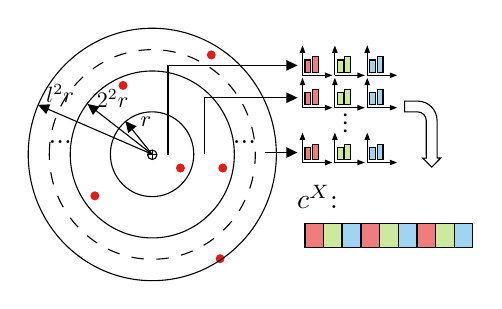
\begin{tikzpicture}[x=0.75pt,y=0.75pt,yscale=-0.6,xscale=0.6]
%uncomment if require: \path (0,300); %set diagram left start at 0, and has height of 300

%Shape: Ellipse [id:dp22042437585940766] 
\draw   (98.77,131.59) .. controls (98.77,112.78) and (113.76,97.53) .. (132.24,97.53) .. controls (150.73,97.53) and (165.71,112.78) .. (165.71,131.59) .. controls (165.71,150.4) and (150.73,165.64) .. (132.24,165.64) .. controls (113.76,165.64) and (98.77,150.4) .. (98.77,131.59) -- cycle ;
%Shape: Ellipse [id:dp5949676512076546] 
\draw   (66.54,131.77) .. controls (66.54,94.75) and (96.03,64.74) .. (132.42,64.74) .. controls (168.8,64.74) and (198.3,94.75) .. (198.3,131.77) .. controls (198.3,168.79) and (168.8,198.8) .. (132.42,198.8) .. controls (96.03,198.8) and (66.54,168.79) .. (66.54,131.77) -- cycle ;
%Shape: Ellipse [id:dp7072370567814422] 
\draw  [dash pattern={on 4.5pt off 4.5pt}] (49.7,131.77) .. controls (49.7,85.29) and (86.73,47.6) .. (132.42,47.6) .. controls (178.1,47.6) and (215.14,85.29) .. (215.14,131.77) .. controls (215.14,178.25) and (178.1,215.94) .. (132.42,215.94) .. controls (86.73,215.94) and (49.7,178.25) .. (49.7,131.77) -- cycle ;
%Shape: Ellipse [id:dp9376040493166226] 
\draw  [color={rgb, 255:red, 255; green, 0; blue, 0 }  ,draw opacity=1 ][fill={rgb, 255:red, 255; green, 0; blue, 0 }  ,fill opacity=1 ] (151.9,142.66) .. controls (151.9,140.92) and (153.29,139.51) .. (155,139.51) .. controls (156.72,139.51) and (158.11,140.92) .. (158.11,142.66) .. controls (158.11,144.41) and (156.72,145.82) .. (155,145.82) .. controls (153.29,145.82) and (151.9,144.41) .. (151.9,142.66) -- cycle ;
%Shape: Ellipse [id:dp6728764854992865] 
\draw  [color={rgb, 255:red, 255; green, 0; blue, 0 }  ,draw opacity=1 ][fill={rgb, 255:red, 255; green, 0; blue, 0 }  ,fill opacity=1 ] (185.9,142.66) .. controls (185.9,140.92) and (187.29,139.51) .. (189.01,139.51) .. controls (190.72,139.51) and (192.11,140.92) .. (192.11,142.66) .. controls (192.11,144.41) and (190.72,145.82) .. (189.01,145.82) .. controls (187.29,145.82) and (185.9,144.41) .. (185.9,142.66) -- cycle ;
%Shape: Ellipse [id:dp1494936101048986] 
\draw  [color={rgb, 255:red, 255; green, 0; blue, 0 }  ,draw opacity=1 ][fill={rgb, 255:red, 255; green, 0; blue, 0 }  ,fill opacity=1 ] (105.85,76.36) .. controls (105.85,74.61) and (107.24,73.2) .. (108.96,73.2) .. controls (110.67,73.2) and (112.06,74.61) .. (112.06,76.36) .. controls (112.06,78.1) and (110.67,79.51) .. (108.96,79.51) .. controls (107.24,79.51) and (105.85,78.1) .. (105.85,76.36) -- cycle ;
%Shape: Ellipse [id:dp5546182167747219] 
\draw  [color={rgb, 255:red, 255; green, 0; blue, 0 }  ,draw opacity=1 ][fill={rgb, 255:red, 255; green, 0; blue, 0 }  ,fill opacity=1 ] (176.69,51.85) .. controls (176.69,50.11) and (178.08,48.69) .. (179.8,48.69) .. controls (181.51,48.69) and (182.9,50.11) .. (182.9,51.85) .. controls (182.9,53.59) and (181.51,55.01) .. (179.8,55.01) .. controls (178.08,55.01) and (176.69,53.59) .. (176.69,51.85) -- cycle ;
%Shape: Ellipse [id:dp20582881370354322] 
\draw  [color={rgb, 255:red, 255; green, 0; blue, 0 }  ,draw opacity=1 ][fill={rgb, 255:red, 255; green, 0; blue, 0 }  ,fill opacity=1 ] (83.19,165.01) .. controls (83.19,163.26) and (84.58,161.85) .. (86.29,161.85) .. controls (88.01,161.85) and (89.4,163.26) .. (89.4,165.01) .. controls (89.4,166.75) and (88.01,168.17) .. (86.29,168.17) .. controls (84.58,168.17) and (83.19,166.75) .. (83.19,165.01) -- cycle ;
%Shape: Ellipse [id:dp35339284724607267] 
\draw  [color={rgb, 255:red, 255; green, 0; blue, 0 }  ,draw opacity=1 ][fill={rgb, 255:red, 255; green, 0; blue, 0 }  ,fill opacity=1 ] (183.78,215.46) .. controls (183.78,213.72) and (185.17,212.3) .. (186.88,212.3) .. controls (188.6,212.3) and (189.99,213.72) .. (189.99,215.46) .. controls (189.99,217.21) and (188.6,218.62) .. (186.88,218.62) .. controls (185.17,218.62) and (183.78,217.21) .. (183.78,215.46) -- cycle ;
%Straight Lines [id:da8440305272338511] 
\draw    (132.38,128.23) -- (132.38,135.8) ;


%Straight Lines [id:da18353521910609616] 
\draw    (128.6,132.02) -- (136.16,132.02) ;


%Straight Lines [id:da6160021318684068] 
\draw    (132.24,131.59) -- (112.09,106.47) ;
\draw [shift={(110.84,104.91)}, rotate = 411.26] [fill={rgb, 255:red, 0; green, 0; blue, 0 }  ][line width=0.75]  [draw opacity=0] (8.93,-4.29) -- (0,0) -- (8.93,4.29) -- cycle    ;

%Straight Lines [id:da4361175020790148] 
\draw    (132.24,131.59) -- (81.95,92.44) ;
\draw [shift={(80.38,91.21)}, rotate = 397.9] [fill={rgb, 255:red, 0; green, 0; blue, 0 }  ][line width=0.75]  [draw opacity=0] (8.93,-4.29) -- (0,0) -- (8.93,4.29) -- cycle    ;

%Straight Lines [id:da2816608379552582] 
\draw    (132.24,131.59) -- (42.54,92.73) ;
\draw [shift={(40.71,91.94)}, rotate = 383.41999999999996] [fill={rgb, 255:red, 0; green, 0; blue, 0 }  ][line width=0.75]  [draw opacity=0] (8.93,-4.29) -- (0,0) -- (8.93,4.29) -- cycle    ;

%Shape: Ellipse [id:dp6312040354242004] 
\draw   (32.8,131.77) .. controls (32.8,75.79) and (77.4,30.41) .. (132.42,30.41) .. controls (187.43,30.41) and (232.03,75.79) .. (232.03,131.77) .. controls (232.03,187.75) and (187.43,233.13) .. (132.42,233.13) .. controls (77.4,233.13) and (32.8,187.75) .. (32.8,131.77) -- cycle ;
%Straight Lines [id:da7388753114522317] 
\draw    (253.03,68.23) -- (253.03,46.23) ;
\draw [shift={(253.03,44.23)}, rotate = 450] [fill={rgb, 255:red, 0; green, 0; blue, 0 }  ][line width=0.75]  [draw opacity=0] (5.93,-2.29) -- (0,0) -- (5.93,2.29) -- cycle    ;

%Straight Lines [id:da4000394565086268] 
\draw    (253.03,68.23) -- (275.03,68.23) ;
\draw [shift={(277.03,68.23)}, rotate = 180] [fill={rgb, 255:red, 0; green, 0; blue, 0 }  ][line width=0.75]  [draw opacity=0] (5.93,-2.29) -- (0,0) -- (5.93,2.29) -- cycle    ;

%Shape: Rectangle [id:dp016947909178976484] 
\draw  [color=black  ,draw opacity=1 ][fill=red  ,fill opacity=0.57 ] (255.03,55.93) -- (259.7,55.93) -- (259.7,65.63) -- (255.03,65.63) -- cycle ;
%Shape: Rectangle [id:dp5625317123053011] 
\draw  [color=black  ,draw opacity=1 ][fill=red  ,fill opacity=0.57 ] (261.03,53.46) -- (265.7,53.46) -- (265.7,65.63) -- (261.03,65.63) -- cycle ;

%Straight Lines [id:da620614004914323] 
\draw    (145.03,132.23) -- (145.03,60.23) ;


%Shape: Circle [id:dp005683642466507988] 
\draw   (128.6,132.02) .. controls (128.6,129.93) and (130.29,128.23) .. (132.38,128.23) .. controls (134.47,128.23) and (136.16,129.93) .. (136.16,132.02) .. controls (136.16,134.11) and (134.47,135.8) .. (132.38,135.8) .. controls (130.29,135.8) and (128.6,134.11) .. (128.6,132.02) -- cycle ;
%Straight Lines [id:da022437387852998092] 
\draw    (145.03,60.23) -- (247.03,60.23) ;
\draw [shift={(249.03,60.23)}, rotate = 180] [fill={rgb, 255:red, 0; green, 0; blue, 0 }  ][line width=0.75]  [draw opacity=0] (8.93,-4.29) -- (0,0) -- (8.93,4.29) -- cycle    ;

%Straight Lines [id:da3327524132297772] 
\draw    (174.03,131.23) -- (174.03,86.23) ;


%Straight Lines [id:da2525359458205172] 
\draw    (279.03,68.23) -- (279.03,46.23) ;
\draw [shift={(279.03,44.23)}, rotate = 450] [fill={rgb, 255:red, 0; green, 0; blue, 0 }  ][line width=0.75]  [draw opacity=0] (5.93,-2.29) -- (0,0) -- (5.93,2.29) -- cycle    ;

%Straight Lines [id:da16414789555797105] 
\draw    (279.03,68.23) -- (301.03,68.23) ;
\draw [shift={(303.03,68.23)}, rotate = 180] [fill={rgb, 255:red, 0; green, 0; blue, 0 }  ][line width=0.75]  [draw opacity=0] (5.93,-2.29) -- (0,0) -- (5.93,2.29) -- cycle    ;

%Shape: Rectangle [id:dp8274809657348666] 
\draw  [color=black  ,draw opacity=1 ][fill=green  ,fill opacity=0.57 ] (281.03,55.93) -- (285.7,55.93) -- (285.7,65.63) -- (281.03,65.63) -- cycle ;
%Shape: Rectangle [id:dp06782765238071065] 
\draw  [color=black  ,draw opacity=1 ][fill=green  ,fill opacity=0.57 ] (287.03,53.46) -- (291.7,53.46) -- (291.7,65.63) -- (287.03,65.63) -- cycle ;
%Straight Lines [id:da04541867871992544] 
\draw    (305.03,68.23) -- (305.03,46.23) ;
\draw [shift={(305.03,44.23)}, rotate = 450] [fill={rgb, 255:red, 0; green, 0; blue, 0 }  ][line width=0.75]  [draw opacity=0] (5.93,-2.29) -- (0,0) -- (5.93,2.29) -- cycle    ;

%Straight Lines [id:da20964508840822693] 
\draw    (305.03,68.23) -- (327.03,68.23) ;
\draw [shift={(329.03,68.23)}, rotate = 180] [fill={rgb, 255:red, 0; green, 0; blue, 0 }  ][line width=0.75]  [draw opacity=0] (5.93,-2.29) -- (0,0) -- (5.93,2.29) -- cycle    ;

%Shape: Rectangle [id:dp6690668435039354] 
\draw  [color=black  ,draw opacity=1 ][fill=skyblue  ,fill opacity=0.57 ] (307.03,55.93) -- (311.7,55.93) -- (311.7,65.63) -- (307.03,65.63) -- cycle ;
%Shape: Rectangle [id:dp9255699869921165] 
\draw  [color=black  ,draw opacity=1 ][fill=skyblue  ,fill opacity=0.57 ] (313.03,53.46) -- (317.7,53.46) -- (317.7,65.63) -- (313.03,65.63) -- cycle ;
%Straight Lines [id:da8165440404194242] 
\draw    (253.03,94.23) -- (253.03,72.23) ;
\draw [shift={(253.03,70.23)}, rotate = 450] [fill={rgb, 255:red, 0; green, 0; blue, 0 }  ][line width=0.75]  [draw opacity=0] (5.93,-2.29) -- (0,0) -- (5.93,2.29) -- cycle    ;

%Straight Lines [id:da29454216862732807] 
\draw    (253.03,94.23) -- (275.03,94.23) ;
\draw [shift={(277.03,94.23)}, rotate = 180] [fill={rgb, 255:red, 0; green, 0; blue, 0 }  ][line width=0.75]  [draw opacity=0] (5.93,-2.29) -- (0,0) -- (5.93,2.29) -- cycle    ;

%Shape: Rectangle [id:dp2984155781668567] 
\draw  [color=black  ,draw opacity=1 ][fill=red  ,fill opacity=0.57 ] (255.03,81.93) -- (259.7,81.93) -- (259.7,91.63) -- (255.03,91.63) -- cycle ;
%Shape: Rectangle [id:dp7229599369299615] 
\draw  [color=black  ,draw opacity=1 ][fill=red  ,fill opacity=0.57 ] (261.03,79.46) -- (265.7,79.46) -- (265.7,91.63) -- (261.03,91.63) -- cycle ;
%Straight Lines [id:da10039448001605955] 
\draw    (279.03,94.23) -- (279.03,72.23) ;
\draw [shift={(279.03,70.23)}, rotate = 450] [fill={rgb, 255:red, 0; green, 0; blue, 0 }  ][line width=0.75]  [draw opacity=0] (5.93,-2.29) -- (0,0) -- (5.93,2.29) -- cycle    ;

%Straight Lines [id:da8722018166510564] 
\draw    (279.03,94.23) -- (301.03,94.23) ;
\draw [shift={(303.03,94.23)}, rotate = 180] [fill={rgb, 255:red, 0; green, 0; blue, 0 }  ][line width=0.75]  [draw opacity=0] (5.93,-2.29) -- (0,0) -- (5.93,2.29) -- cycle    ;

%Shape: Rectangle [id:dp5710893991029787] 
\draw  [color=black  ,draw opacity=1 ][fill=green  ,fill opacity=0.57 ] (281.03,81.93) -- (285.7,81.93) -- (285.7,91.63) -- (281.03,91.63) -- cycle ;
%Shape: Rectangle [id:dp9056928866973952] 
\draw  [color=black  ,draw opacity=1 ][fill=green  ,fill opacity=0.57 ] (287.03,79.46) -- (291.7,79.46) -- (291.7,91.63) -- (287.03,91.63) -- cycle ;
%Straight Lines [id:da48015611435891126] 
\draw    (305.03,94.23) -- (305.03,72.23) ;
\draw [shift={(305.03,70.23)}, rotate = 450] [fill={rgb, 255:red, 0; green, 0; blue, 0 }  ][line width=0.75]  [draw opacity=0] (5.93,-2.29) -- (0,0) -- (5.93,2.29) -- cycle    ;

%Straight Lines [id:da21508790577080394] 
\draw    (305.03,94.23) -- (327.03,94.23) ;
\draw [shift={(329.03,94.23)}, rotate = 180] [fill={rgb, 255:red, 0; green, 0; blue, 0 }  ][line width=0.75]  [draw opacity=0] (5.93,-2.29) -- (0,0) -- (5.93,2.29) -- cycle    ;

%Shape: Rectangle [id:dp656328402305677] 
\draw  [color=black  ,draw opacity=1 ][fill=skyblue  ,fill opacity=0.57 ] (307.03,81.93) -- (311.7,81.93) -- (311.7,91.63) -- (307.03,91.63) -- cycle ;
%Shape: Rectangle [id:dp5664134518061891] 
\draw  [color=black  ,draw opacity=1 ][fill=skyblue  ,fill opacity=0.57 ] (313.03,79.46) -- (317.7,79.46) -- (317.7,91.63) -- (313.03,91.63) -- cycle ;
%Straight Lines [id:da26856630441769913] 
\draw    (253.03,138.23) -- (253.03,116.23) ;
\draw [shift={(253.03,114.23)}, rotate = 450] [fill={rgb, 255:red, 0; green, 0; blue, 0 }  ][line width=0.75]  [draw opacity=0] (5.93,-2.29) -- (0,0) -- (5.93,2.29) -- cycle    ;

%Straight Lines [id:da045342033266806414] 
\draw    (253.03,138.23) -- (275.03,138.23) ;
\draw [shift={(277.03,138.23)}, rotate = 180] [fill={rgb, 255:red, 0; green, 0; blue, 0 }  ][line width=0.75]  [draw opacity=0] (5.93,-2.29) -- (0,0) -- (5.93,2.29) -- cycle    ;

%Shape: Rectangle [id:dp21465817035357382] 
\draw  [color=black  ,draw opacity=1][fill=red  ,fill opacity=0.57 ] (255.03,125.93) -- (259.7,125.93) -- (259.7,135.63) -- (255.03,135.63) -- cycle ;
%Shape: Rectangle [id:dp6836107840104558] 
\draw  [color=black  ,draw opacity=1][fill=red  ,fill opacity=0.57 ] (261.03,123.46) -- (265.7,123.46) -- (265.7,135.63) -- (261.03,135.63) -- cycle ;
%Straight Lines [id:da7152252219644601] 
\draw    (279.03,138.23) -- (279.03,116.23) ;
\draw [shift={(279.03,114.23)}, rotate = 450] [fill={rgb, 255:red, 0; green, 0; blue, 0 }  ][line width=0.75]  [draw opacity=0] (5.93,-2.29) -- (0,0) -- (5.93,2.29) -- cycle    ;

%Straight Lines [id:da9384291951491641] 
\draw    (279.03,138.23) -- (301.03,138.23) ;
\draw [shift={(303.03,138.23)}, rotate = 180] [fill={rgb, 255:red, 0; green, 0; blue, 0 }  ][line width=0.75]  [draw opacity=0] (5.93,-2.29) -- (0,0) -- (5.93,2.29) -- cycle    ;

%Shape: Rectangle [id:dp30291585437230484] 
\draw  [color=black  ,draw opacity=1][fill=green  ,fill opacity=0.57 ] (281.03,125.93) -- (285.7,125.93) -- (285.7,135.63) -- (281.03,135.63) -- cycle ;
%Shape: Rectangle [id:dp8268094585264629] 
\draw  [color=black  ,draw opacity=1][fill=green  ,fill opacity=0.57 ] (287.03,123.46) -- (291.7,123.46) -- (291.7,135.63) -- (287.03,135.63) -- cycle ;
%Straight Lines [id:da6298730087940589] 
\draw    (305.03,138.23) -- (305.03,116.23) ;
\draw [shift={(305.03,114.23)}, rotate = 450] [fill={rgb, 255:red, 0; green, 0; blue, 0 }  ][line width=0.75]  [draw opacity=0] (5.93,-2.29) -- (0,0) -- (5.93,2.29) -- cycle    ;

%Straight Lines [id:da3708666876743798] 
\draw    (305.03,138.23) -- (327.03,138.23) ;
\draw [shift={(329.03,138.23)}, rotate = 180] [fill={rgb, 255:red, 0; green, 0; blue, 0 }  ][line width=0.75]  [draw opacity=0] (5.93,-2.29) -- (0,0) -- (5.93,2.29) -- cycle    ;

%Shape: Rectangle [id:dp00038976604596641096] 
\draw  [color=black  ,draw opacity=1][fill=skyblue  ,fill opacity=0.57 ] (307.03,125.93) -- (311.7,125.93) -- (311.7,135.63) -- (307.03,135.63) -- cycle ;
%Shape: Rectangle [id:dp36800166267960555] 
\draw  [color=black  ,draw opacity=1][fill=skyblue  ,fill opacity=0.57 ] (313.03,123.46) -- (317.7,123.46) -- (317.7,135.63) -- (313.03,135.63) -- cycle ;
%Straight Lines [id:da7693768627138445] 
\draw    (174.03,86.23) -- (247.03,86.23) ;
\draw [shift={(249.03,86.23)}, rotate = 180] [fill={rgb, 255:red, 0; green, 0; blue, 0 }  ][line width=0.75]  [draw opacity=0] (8.93,-4.29) -- (0,0) -- (8.93,4.29) -- cycle    ;

%Straight Lines [id:da607729095409385] 
\draw    (223.03,130.23) -- (247.03,130.23) ;
\draw [shift={(249.03,130.23)}, rotate = 180] [fill={rgb, 255:red, 0; green, 0; blue, 0 }  ][line width=0.75]  [draw opacity=0] (8.93,-4.29) -- (0,0) -- (8.93,4.29) -- cycle    ;

%Shape: Rectangle [id:dp8711908392617309] 
\draw  [fill=red ,fill opacity=0.57 ] (255,187.23) -- (269.77,187.23) -- (269.77,206.14) -- (255,206.14) -- cycle ;
%Shape: Rectangle [id:dp18481612105128353] 
\draw  [fill=green  ,fill opacity=0.57 ] (270,187.23) -- (284.77,187.23) -- (284.77,206.14) -- (270,206.14) -- cycle ;
%Shape: Rectangle [id:dp7615959072987122] 
\draw  [fill=skyblue  ,fill opacity=0.57 ] (285,187.23) -- (299.77,187.23) -- (299.77,206.14) -- (285,206.14) -- cycle ;
%Shape: Rectangle [id:dp1813533709159073] 
\draw  [fill=red ,fill opacity=0.57 ] (300,187.23) -- (314.77,187.23) -- (314.77,206.14) -- (300,206.14) -- cycle ;
%Shape: Rectangle [id:dp8129375218164283] 
\draw  [fill=green  ,fill opacity=0.57 ] (315,187.23) -- (329.77,187.23) -- (329.77,206.14) -- (315,206.14) -- cycle ;
%Shape: Rectangle [id:dp9302976015184905] 
\draw  [fill=skyblue  ,fill opacity=0.57 ] (330,187.23) -- (344.77,187.23) -- (344.77,206.14) -- (330,206.14) -- cycle ;
%Shape: Rectangle [id:dp3052728377366358] 
\draw  [fill=red  ,fill opacity=0.57 ] (345,187.23) -- (359.77,187.23) -- (359.77,206.14) -- (345,206.14) -- cycle ;
%Shape: Rectangle [id:dp9806675697084216] 
\draw  [fill=green  ,fill opacity=0.57 ] (360,187.23) -- (374.77,187.23) -- (374.77,206.14) -- (360,206.14) -- cycle ;
%Shape: Rectangle [id:dp526916695713156] 
\draw  [fill=skyblue  ,fill opacity=0.57 ] (375,187.23) -- (389.77,187.23) -- (389.77,206.14) -- (375,206.14) -- cycle ;

%Bend Arrow [id:dp941959923921848] 
\draw   (335.03,88.93) -- (345.45,88.92) .. controls (354.07,88.91) and (361.08,95.89) .. (361.09,104.52) -- (361.13,134.65) -- (364.02,134.64) -- (356.8,141.94) -- (349.56,134.66) -- (352.45,134.66) -- (352.41,104.53) .. controls (352.41,100.7) and (349.29,97.59) .. (345.46,97.6) -- (335.05,97.61) -- cycle ;

% Text Node
\draw (206.44,121.76) node  [scale=1] {...};
% Text Node
\draw (58.44,121.76) node  [scale=1] {...};
% Text Node
\draw (100.64,86.72) node [scale=0.8]  {$2^{2} r$};
% Text Node
\draw (127.27,105.46) node [scale=0.8]  {$r$};
% Text Node
\draw (58.43,83.12) node [scale=0.8]  {$l^{2} r$};
% Text Node
\draw (287.44,106.76) node [rotate=-90] [align=left] {...};
% Text Node
\draw (265,165.6) node   {$\boldsymbol{c}^{X}$:};

\end{tikzpicture}

			\caption{\centering \footnotesize Computing the color signature $\boldsymbol{c}^X$.}
			\label{fig:color-signature}	
		\end{figure}
		\end{center}
	\end{column}
	\end{columns}	
}

\frame{
	\frametitle{Signature Vector}
	\begin{columns}
	\begin{column}{0.5\textwidth}
		\begin{itemize}
			\justifying
			\item Both $\boldsymbol{s}^X$ and $\boldsymbol{c}^X$ are normalized and concatenated into a single signature vector;
			\item The signature matrix $\boldsymbol{A}$ is augmented by a row with the concatenated vector.
		\end{itemize}
	\end{column}
	\begin{column}{0.5\textwidth}  %%<--- here
		\begin{center}
		\begin{figure}[h!]
			\centering
			\vspace{0.7cm}
			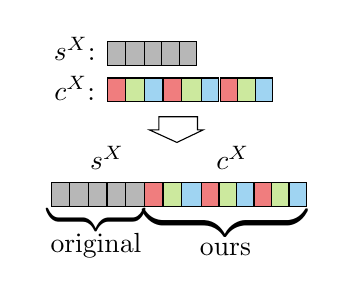
\begin{tikzpicture}[x=0.75pt,y=0.75pt,yscale=-0.6,xscale=0.6]
%uncomment if require: \path (0,300); %set diagram left start at 0, and has height of 300

%Shape: Rectangle [id:dp056770282484357115] 
\draw  [fill=grey  ,fill opacity=0.57 ] (133,39.23) -- (146.77,39.23) -- (146.77,58.14) -- (133,58.14) -- cycle ;
%Shape: Rectangle [id:dp8374236504797968] 
\draw  [fill=grey  ,fill opacity=0.57 ] (147,39.23) -- (160.77,39.23) -- (160.77,58.14) -- (147,58.14) -- cycle ;
%Shape: Rectangle [id:dp8517953159568432] 
\draw  [fill=grey  ,fill opacity=0.57 ] (161,39.23) -- (174.77,39.23) -- (174.77,58.14) -- (161,58.14) -- cycle ;
%Shape: Rectangle [id:dp797061078463292] 
\draw  [fill=grey  ,fill opacity=0.57 ] (103,39.23) -- (117.77,39.23) -- (117.77,58.14) -- (103,58.14) -- cycle ;
%Shape: Rectangle [id:dp12299147827719992] 
\draw  [fill=grey  ,fill opacity=0.57 ] (118,39.23) -- (132.77,39.23) -- (132.77,58.14) -- (118,58.14) -- cycle ;

%Shape: Rectangle [id:dp8711908392617309] 
\draw  [fill=red ,fill opacity=0.57 ] (194,68.23) -- (207.77,68.23) -- (207.77,87.14) -- (194,87.14) -- cycle ;
%Shape: Rectangle [id:dp18481612105128353] 
\draw  [fill=green  ,fill opacity=0.57 ] (208,68.23) -- (221.77,68.23) -- (221.77,87.14) -- (208,87.14) -- cycle ;
%Shape: Rectangle [id:dp7615959072987122] 
\draw  [fill=skyblue  ,fill opacity=0.57 ] (222,68.23) -- (235.77,68.23) -- (235.77,87.14) -- (222,87.14) -- cycle ;
%Shape: Rectangle [id:dp1813533709159073] 
\draw  [fill=red ,fill opacity=0.57 ] (103,68.23) -- (117.77,68.23) -- (117.77,87.14) -- (103,87.14) -- cycle ;
%Shape: Rectangle [id:dp8129375218164283] 
\draw  [fill=green  ,fill opacity=0.57 ] (118,68.23) -- (132.77,68.23) -- (132.77,87.14) -- (118,87.14) -- cycle ;
%Shape: Rectangle [id:dp9302976015184905] 
\draw  [fill=skyblue  ,fill opacity=0.57 ] (133,68.23) -- (147.77,68.23) -- (147.77,87.14) -- (133,87.14) -- cycle ;
%Shape: Rectangle [id:dp3052728377366358] 
\draw  [fill=red  ,fill opacity=0.57 ] (148,68.23) -- (162.77,68.23) -- (162.77,87.14) -- (148,87.14) -- cycle ;
%Shape: Rectangle [id:dp9806675697084216] 
\draw  [fill=green  ,fill opacity=0.57 ] (163,68.23) -- (178.77,68.23) -- (178.77,87.14) -- (163,87.14) -- cycle ;
%Shape: Rectangle [id:dp526916695713156] 
\draw  [fill=skyblue  ,fill opacity=0.57 ] (179,68.23) -- (192.77,68.23) -- (192.77,87.14) -- (179,87.14) -- cycle ;

%Down Arrow [id:dp6057459970471565] 
\draw   (137,109.95) -- (144.51,109.95) -- (144.51,99.37) -- (175.52,99.37) -- (175.52,109.95) -- (180.03,109.95) -- (159.02,120) -- cycle ;

%Shape: Rectangle [id:dp056770282484357115] 
\draw  [fill=grey  ,fill opacity=0.57 ] (58,152.23) -- (72.77,152.23) -- (72.77,171.14) -- (58,171.14) -- cycle ;
%Shape: Rectangle [id:dp8374236504797968] 
\draw  [fill=grey  ,fill opacity=0.57 ] (73,152.23) -- (87.77,152.23) -- (87.77,171.14) -- (73,171.14) -- cycle ;
%Shape: Rectangle [id:dp8517953159568432] 
\draw  [fill=grey  ,fill opacity=0.57 ] (88,152.23) -- (102.77,152.23) -- (102.77,171.14) -- (88,171.14) -- cycle ;
%Shape: Rectangle [id:dp797061078463292] 
\draw  [fill=grey  ,fill opacity=0.57 ] (103,152.23) -- (117.77,152.23) -- (117.77,171.14) -- (103,171.14) -- cycle ;
%Shape: Rectangle [id:dp12299147827719992] 
\draw  [fill=grey  ,fill opacity=0.57 ] (118,152.23) -- (132.77,152.23) -- (132.77,171.14) -- (118,171.14) -- cycle ;
%Shape: Rectangle [id:dp8711908392617309] 
\draw  [fill=red ,fill opacity=0.57 ] (133,152.23) -- (147.77,152.23) -- (147.77,171.14) -- (133,171.14) -- cycle ;
%Shape: Rectangle [id:dp18481612105128353] 
\draw  [fill=green  ,fill opacity=0.57 ] (148,152.23) -- (162.77,152.23) -- (162.77,171.14) -- (148,171.14) -- cycle ;
%Shape: Rectangle [id:dp7615959072987122] 
\draw  [fill=skyblue  ,fill opacity=0.57 ] (163,152.23) -- (178.77,152.23) -- (178.77,171.14) -- (163,171.14) -- cycle ;
%Shape: Rectangle [id:dp1813533709159073] 
\draw  [fill=red ,fill opacity=0.57 ] (179,152.23) -- (192.77,152.23) -- (192.77,171.14) -- (179,171.14) -- cycle ;
%Shape: Rectangle [id:dp8129375218164283] 
\draw  [fill=green  ,fill opacity=0.57 ] (193,152.23) -- (206.77,152.23) -- (206.77,171.14) -- (193,171.14) -- cycle ;
%Shape: Rectangle [id:dp9302976015184905] 
\draw  [fill=skyblue  ,fill opacity=0.57 ] (207,152.23) -- (220.77,152.23) -- (220.77,171.14) -- (207,171.14) -- cycle ;
%Shape: Rectangle [id:dp3052728377366358] 
\draw  [fill=red  ,fill opacity=0.57 ] (221,152.23) -- (234.77,152.23) -- (234.77,171.14) -- (221,171.14) -- cycle ;
%Shape: Rectangle [id:dp9806675697084216] 
\draw  [fill=green  ,fill opacity=0.57 ] (235,152.23) -- (248.77,152.23) -- (248.77,171.14) -- (235,171.14) -- cycle ;
%Shape: Rectangle [id:dp526916695713156] 
\draw  [fill=skyblue  ,fill opacity=0.57 ] (249,152.23) -- (262.77,152.23) -- (262.77,171.14) -- (249,171.14) -- cycle ;

% Text Node
\draw (77,44.6) node   {$\boldsymbol{s}^{X}$:};
% Text Node
\draw (77,76.6) node   {$\boldsymbol{c}^{X}$:};
% Text Node
\draw (103,132.6) node   {$\boldsymbol{s}^{X}$};
% Text Node
\draw (204,132.6) node   {$\boldsymbol{c}^{X}$};
% Text Node
\draw (94,182) node [scale=2.0,rotate=-270] [align=left] {\Big\{};
% Text Node
\draw (198,185) node [scale=2.0,rotate=-270] [align=left] {\Bigg\{};
% Text Node
\draw (94,202.65) node  [align=left] {original};
% Text Node
\draw (198,205.65) node  [align=left] {ours};


\end{tikzpicture}

			\caption{\centering \footnotesize Concatenated shape and color signatures.}
			\label{fig:projection-signature}	
		\end{figure}
		\end{center}
	\end{column}
	\end{columns}	
}

\frame{
	\frametitle{Dimensionality Reduction}
	\begin{itemize}
		\justifying
		\item For every 2D projection, both shape and color signatures are computed, concatenated and included into $\boldsymbol{A}$;
		\item SVD of $\boldsymbol{A}$ is computed, with the resulting 1st left and right singular vectors being concatenated and used as the final descriptor.
	\end{itemize}
}

\section{Loop Closure Detection}
\frame{
	\frametitle{Pipeline}
	\begin{itemize}
		\justifying
		\item Compute a descriptor for each point cloud and query them against the database:
		\begin{itemize}
			\justifying
			\item Brute-force matching approach using the $L2$ norm;
			%\item Current and adjacent frames are excluded to avoid self-queries;			
			%pensar sobre como explicar essa janela (img, ...)
			\item Detection comes down to finding the most similar descriptor under a predefined threshold (later used for PR curves).
		\end{itemize}
	\end{itemize}
}

\section{Dataset Sequences}
\frame{
	\frametitle{Point Clouds}
	\begin{itemize}
		\justifying			
		\item KITTI\footnote[frame]{\tiny (GEIGER; LENZ; URTASUN, 2012)} sequences 00, 05, 06 and 07 were used:
		\begin{itemize}
			\justifying
			\item 3D LIDAR with $360^{\circ}$ FoV, and a forward facing stereo color camera system, providing synchronized frames and rectified images;
		\end{itemize}
		\item For each sequence, we generated semi-dense and dense point clouds offline, using sensors readings and public available tools;		
	\end{itemize}
}

\frame{
	\frametitle{Camera-LIDAR Sensor Fusion}
	\begin{columns}
	\begin{column}{0.5\textwidth}
		\begin{itemize}
			\justifying
			\item kitti\_lidar\_camera\footnote[frame]{\tiny https://github.com/LidarPerception/kitti\_lidar\_camera} package (ROS) was used:
			\begin{itemize}
				\justifying
				\item LIDAR limited to forward facing FoV;  
				\item 3D points were projected onto 2D image, associating color values.
			\end{itemize}
		\end{itemize}
	\end{column}
	\begin{column}{0.5\textwidth}  %%<--- here
		\begin{center}
		\begin{figure}[h!]
			\centering
			\includegraphics[height=2cm, width=\textwidth]{lidarprojected.png}
			\caption{\centering \footnotesize 3D LIDAR points projected on 2D image. Frame from the KITTI odometry dataset.}
			\label{fig:camera-lidar-fusion}
		\end{figure}
		\end{center}
	\end{column}
	\end{columns}	
}

\frame{
	\frametitle{Stereo Depth Estimation}
	\begin{columns}
	\begin{column}{0.5\textwidth}
		\begin{itemize}
			\justifying
			\item image\_undistort\footnote[frame]{\tiny https://github.com/ethz-asl/image\_undistort} package (ROS) was used:
			\begin{itemize}
				\justifying
				\item Employs block matching technique from OpenCV\footnote[frame]{\tiny https://opencv.org/};
				\item Point clouds generated using default parameters for KITTI sequences.
			\end{itemize}
		\end{itemize}
	\end{column}
	\begin{column}{0.5\textwidth}  %%<--- here
		\begin{center}
		\begin{figure}[h!]
			\centering
			\includegraphics[height=2cm, width=\textwidth]{stereodepth.png}
			\caption{\centering \footnotesize Depth estimated from stereo camera. Frame from the KITTI odometry dataset.}
			\label{fig:stereo-depth}
		\end{figure}
		\end{center}
	\end{column}
	\end{columns}
}

\section{Experiments}
\frame{
	\frametitle{Our platform}
	\begin{itemize}
		\justifying
		\item Laptop Intel i7 quad-core 2.00 GHz CPU and 8 GB RAM;
		\item Both M2DP and c-M2DP were implemented in C++, using PCL\footnote[frame]{\tiny http://pointclouds.org} and Eigen\footnote[frame]{\tiny http://eigen.tuxfamily.org/};
		\item In order to compare our results, we used the global variant of the CSHOT descriptor provided by PCL.
	\end{itemize}
}

\frame{
	\frametitle{Parameters}
	\begin{columns}
		\begin{column}{0.5\textwidth}
			\begin{itemize}
				\justifying
				\item M2DP and c-M2DP parameters were the same from original work;
				%%PENSAR EM COMO APRESENTAR ISSO:
				\item c-M2DP color bins parameter was set as $g = h$; % and $w = 3$ (RGB, HSV and CIELab); 
			\end{itemize}
		\end{column}
		\begin{column}{0.5\textwidth}  %%<--- here
			\begin{center}
				\begin{table}[h!]
					\footnotesize
					\centering
					\caption{M2DP and c-M2DP Parameters}
					\label{tab:settings}
					\begin{tabularx}{\textwidth}{@{}lcc@{}}\hline
						\textbf{Parameter} & \textbf{M2DP} & \textbf{c-M2DP} \\ \hline	
						Azim. angles ($b$) & $4$ & $4$ \\
						Elev. angles ($q$) & $16$ & $16$ \\	
						Conc. circles ($l$) & $8$ & $8$ \\
						Shape bins ($h$) & $16$ & $16$ \\ 
						Color bins ($g$) & - & $16$ \\ \hline
						\textbf{Vector length} & $192$ & $576$ \\ \hline
					\end{tabularx}
				\end{table}
			\end{center}
		\end{column}
	\end{columns}	
}	

\frame{
	\frametitle{Parameters}
	\begin{itemize}
		\justifying
		\item CSHOT default parameters from PCL (vector length: $1344$);
		\item Normals are estimated for CSHOT using the neighborhood around each point, requiring a radius parameter:
		\begin{itemize}
			\justifying
			\item It can be insufficient, generating invalid results, or be a costly process due to the amount of points; 
			\item Before each sequence, using the 1st frame:
			\begin{itemize}
				\justifying
				\item Radius was set as 5 times the average distance of the nearest point.
			\end{itemize}
		\end{itemize}			
	\end{itemize}
}	

%\frame{
	%\frametitle{Parameters}
	%\begin{itemize}
		%\justifying
		%\item In the loop closure detection pipeline, parameters were the same from original work:
		%\begin{itemize}
			%\justifying		
			%\item Self-queries are avoided using $\pm50$ window;
			%\item Two locations are considered as the ground truth loop closure if their distance is $<10m$.
			%A loop closure is considered correct if the matched point clouds are $<10m$ from each other in the ground-truth trajectory.
			%\item Detected loop closures are considered ground-truth if $<10m$ of the exact location in the trajectory.			
		%\end{itemize}
	%\end{itemize}
%}	

\frame{
	\frametitle{Evaluation}
	\begin{itemize}
		\justifying
		\item Times to compute each descriptor and perform the matching process were measured;
		\item Precision-recall curves were generated by varying the descriptor similarity threshold:
		\begin{itemize}
			\justifying
			\item Two locations are considered as the ground truth loop closure if their distance is $<10m$;
		\end{itemize}
		%\begin{itemize}
		%	\justifying
		%	\item Loop closures are considered GT if $<10m$ in the trajectory;						
		%\end{itemize}
		\item Recall rates at $100\%$ precision are highlighted:
		\begin{itemize}
			\justifying
			\item False loop closures are catastrophic for the map building and can be irrecoverable for SLAM.
		\end{itemize}					
	\end{itemize}
}

\frame{
	\frametitle{Evaluation}
	\begin{itemize}
		\justifying
		\item At first, we evaluated each descriptor with semi-dense clouds, generated through camera-LIDAR fusion;
		\item After that, we experimented with more dense clouds, generated through stereo depth estimation.		
		%\item We evaluated each descriptor while using point clouds with distinct densities:
		%\begin{itemize}
			%\justifying
			%\item At first, our experiments were done with semi-dense clouds, generated through camera-LIDAR fusion;
			%\item Our first experiments were done using point clouds sequences generated through camera-LIDAR fusion;
			%\item After that, we experimented using c-M2DP and M2DP with more dense clouds, generated through depth estimation.
			%\item We also evaluate c-M2DP and M2DP using stereo-based sequences:
			%\item In stereo-based sequences:
			
			%\item Evaluate M2DP and c-M2DP results for point clouds generated using a different sensor;
			%\item CSHOT was expected to have better accuracy, but at higher computational costs.
		%\end{itemize}		
	\end{itemize}		
}

\section{Results}
\frame{
	\frametitle{\MakeLowercase{c}-M2DP Color Space}
	\begin{columns}
		\begin{column}{0.5\textwidth}
			\begin{itemize}
				\justifying
				\item c-M2DP color space was chosen after evaluating it using RGB, HSV and CIELab.
				\begin{table}[h!]
					\footnotesize
					\label{tab:100colorspaces}
					\begin{tabularx}{\textwidth}{@{}lcc@{}}\hline
						\textbf{Color Space} & 
						\multicolumn{2}{>{\hsize=\dimexpr2\hsize+2\tabcolsep+\arrayrulewidth\relax}c}{\textbf{Recall Rates}} \\
						& \textbf{Pr. $\mathbf{100\%}$} & \textbf{Pr. $\mathbf{90\%}$} \\ \hline	
						RGB & $\mathbf{82.5\%}$ & $89.2\%$ \\
						HSV & $71.4\%$ & $91.5\%$ \\	
						CIELab & $49.8\%$ & $86.8\%$ \\ \hline
					\end{tabularx}
				\end{table}
			\end{itemize}
		\end{column}
		\begin{column}{0.5\textwidth}  %%<--- here
			\begin{center}
				\begin{figure}[h!]
					\centering
					\begin{tikzpicture}
					\begin{axis}[precision recall color, legend pos=south west]
					\addplot+[] table [x=x, y=y, col sep=semicolon] {"../paper/data/lidar_camera/cm2dp/lab/precisionrecall_kitti06_lidar_camera_cm2dp.csv"};
					\addplot+[] table [x=x, y=y, col sep=semicolon] {"../paper/data/lidar_camera/cm2dp/hsv/precisionrecall_kitti06_lidar_camera_cm2dp.csv"};
					\addplot+[] table [x=x, y=y, col sep=semicolon] {"../paper/data/lidar_camera/cm2dp/rgb/precisionrecall_kitti06_lidar_camera_cm2dp.csv"};
					\legend{Lab, HSV, RGB}
					\end{axis}
					\end{tikzpicture}
					\caption{\centering \footnotesize KITTI 06 camera-LIDAR.}
					\label{fig:color-spaces}	
				\end{figure}
			\end{center}
		\end{column}
	\end{columns}	
}

\frame{
	\frametitle{Time Efficiency}
	\begin{itemize}
		\justifying
		\item In camera-LIDAR sequences:
		\begin{itemize}
			\justifying		
			\item c-M2DP computing time is only $\mathbf{23.2}\%$ higher than M2DP; 
			\item c-M2DP is $\mathbf{22.6}\%$ faster to compute than CSHOT.
		\end{itemize}
	\end{itemize}
	\begin{center}
		\begin{table}[h!]
			\centering
			\footnotesize
			%\caption{Average times computing and matching a descriptor.}
			\label{tab:times-camera-lidar}	
			\begin{tabularx}{\textwidth}{@{}XXX@{}}\hline
				\textbf{Descriptor} & \textbf{Computing ($s$)} & \textbf{Matching ($s$)} \\ \hline
				M2DP & $\mathbf{0.0674}\pm0.0041$ & $\mathbf{0.0043}\pm0.0004$ \\
				c-M2DP* & $\mathbf{0.0830}\pm0.0052$ & $\mathbf{0.0051}\pm0.0006$ \\
				CSHOT & $0.1072\pm0.0168$ & $0.0059\pm0.0005$ \\ \hline
				\tiny *Ours
			\end{tabularx}
		\end{table}					
	\end{center}	
}

\frame{
	\frametitle{Precision-Recall Camera-LIDAR}
	\begin{columns}
		\begin{column}{0.5\textwidth}
			\begin{table}[h!]
				\footnotesize
				\label{tab:100cameralidar06}
				\begin{tabularx}{\textwidth}{@{}lcc@{}}\hline
					\textbf{Descriptor} & 
					\multicolumn{2}{>{\hsize=\dimexpr2\hsize+2\tabcolsep+\arrayrulewidth\relax}c}{\textbf{Recall Rates}} \\
					& \textbf{Pr. $\mathbf{100\%}$} & \textbf{Pr. $\mathbf{90\%}$} \\ \hline
					c-M2DP* & $\mathbf{82.5\%}$ & $89.2\%$ \\
					M2DP & $66.8\%$ & $82.1\%$ \\	
					CSHOT & $81.9\%$ & $90.6\%$ \\ \hline
					\tiny *Ours			
				\end{tabularx}
			\end{table}
			\begin{figure}
				\label{figure:cl06}
				\includegraphics[height=100pt, width=0.8\textwidth]{06.png}
			\end{figure}				
		\end{column}
		\begin{column}{0.5\textwidth}  %%<--- here
			\begin{center}
				\begin{figure}[h!]
					\centering
					\begin{tikzpicture}
					\begin{axis}[precision recall normal, legend pos=south west]
					\addplot+[] table [x=x, y=y, col sep=semicolon] {"../paper/data/lidar_camera/m2dp/precisionrecall_kitti06_lidar_camera_m2dp.csv"};
					\addplot+[] table [x=x, y=y, col sep=semicolon]
					{"../paper/data/lidar_camera/cshot/precisionrecall_kitti06_lidar_camera_cshot.csv"};
					\addplot+[] table [x=x, y=y, col sep=semicolon] {"../paper/data/lidar_camera/cm2dp/rgb/precisionrecall_kitti06_lidar_camera_cm2dp.csv"};  	
					\legend{M2DP, CSHOT, c-M2DP}
					\end{axis}
					\end{tikzpicture}
					\caption{\centering \footnotesize KITTI 06 camera-LIDAR.}
					\label{fig:pr-camera-lidar-06}
				\end{figure}				
			\end{center}
		\end{column}
	\end{columns}	
}

\frame{
	\frametitle{Precision-Recall Camera-LIDAR}
	\begin{columns}
	\begin{column}{0.5\textwidth}
		\begin{table}[h!]
		\footnotesize
		\label{tab:100cameralidar05}
		\begin{tabularx}{\textwidth}{@{}lcc@{}}\hline
			\textbf{Descriptor} & 
			\multicolumn{2}{>{\hsize=\dimexpr2\hsize+2\tabcolsep+\arrayrulewidth\relax}c}{\textbf{Recall Rates}} \\
			& \textbf{Pr. $\mathbf{100\%}$} & \textbf{Pr. $\mathbf{90\%}$} \\ \hline	
			c-M2DP* & $\mathbf{70.9\%}$ & $76.5\%$ \\
			M2DP & $40.9\%$ & $78.2\%$ \\	
			CSHOT & $\mathbf{70.8\%}$ & $83.5\%$ \\ \hline
			\tiny *Ours
		\end{tabularx}
		\end{table}
		\begin{figure}
			\label{figure:cl05}
			\includegraphics[height=100pt, width=0.8\textwidth]{05.png}
		\end{figure}
	\end{column}
	\begin{column}{0.5\textwidth}  %%<--- here
		\begin{center}
		\begin{figure}[h!]
			\centering
			\begin{tikzpicture}
			\begin{axis}[precision recall normal, legend pos=south west]
			\addplot+[] table [x=x, y=y, col sep=semicolon] {"../paper/data/lidar_camera/m2dp/precisionrecall_kitti05_lidar_camera_m2dp.csv"};
			\addplot+[] table [x=x, y=y, col sep=semicolon]
			{"../paper/data/lidar_camera/cshot/precisionrecall_kitti05_lidar_camera_cshot.csv"};
			\addplot+[] table [x=x, y=y, col sep=semicolon] {"../paper/data/lidar_camera/cm2dp/rgb/precisionrecall_kitti05_lidar_camera_cm2dp.csv"};  	
			\legend{M2DP, CSHOT, c-M2DP}
			\end{axis}
			\end{tikzpicture}
			\caption{\centering \footnotesize KITTI 05 camera-LIDAR.}
			\label{fig:pr-camera-lidar-05}
		\end{figure}				
		\end{center}
	\end{column}
	\end{columns}	
}

\frame{
	\frametitle{Precision-Recall Camera-LIDAR}
	\begin{columns}
		\begin{column}{0.5\textwidth}
			\begin{table}[h!]
				\footnotesize
				\label{tab:100cameralidar00}
				\begin{tabularx}{\textwidth}{@{}lcc@{}}\hline
					\textbf{Descriptor} & 
					\multicolumn{2}{>{\hsize=\dimexpr2\hsize+2\tabcolsep+\arrayrulewidth\relax}c}{\textbf{Recall Rates}} \\
					& \textbf{Pr. $\mathbf{100\%}$} & \textbf{Pr. $\mathbf{90\%}$} \\ \hline	
					c-M2DP* & $67.3\%$ & $85.4\%$ \\
					M2DP & $57.4\%$ & $78.2\%$ \\	
					CSHOT & $\mathbf{79.2\%}$ & $88.6\%$ \\ \hline
					\tiny *Ours
				\end{tabularx}
			\end{table}
			\begin{figure}
				\label{figure:cl00}
				\includegraphics[height=100pt, width=0.8\textwidth]{00.png}
			\end{figure}
			
		\end{column}
		\begin{column}{0.5\textwidth}  %%<--- here
			\begin{center}
				\begin{figure}[h!]
					\centering
					\begin{tikzpicture}
					\begin{axis}[precision recall normal, legend pos=south west]
					\addplot+[] table [x=x, y=y, col sep=semicolon] {"../paper/data/lidar_camera/m2dp/precisionrecall_kitti00_lidar_camera_m2dp.csv"};
					\addplot+[] table [x=x, y=y, col sep=semicolon]
					{"../paper/data/lidar_camera/cshot/precisionrecall_kitti00_lidar_camera_cshot.csv"};
					\addplot+[] table [x=x, y=y, col sep=semicolon] {"../paper/data/lidar_camera/cm2dp/rgb/precisionrecall_kitti00_lidar_camera_cm2dp.csv"};  	
					\legend{M2DP, CSHOT, c-M2DP}
					\end{axis}
					\end{tikzpicture}
					\caption{\centering \footnotesize KITTI 00 camera-LIDAR.}
					\label{fig:pr-camera-lidar-00}
				\end{figure}				
			\end{center}
		\end{column}
	\end{columns}	
}

\frame{
	\frametitle{Precision-Recall Camera-LIDAR}
	\begin{columns}
	\begin{column}{0.5\textwidth}
		\begin{table}[h!]
		\footnotesize
		\label{tab:100cameralidar07}
		\begin{tabularx}{\textwidth}{@{}XX@{}}\hline
		\textbf{Descriptor} & \textbf{Recall Rates} \\
		& \textbf{Pr. $\mathbf{100\%}$} \\ \hline	
		c-M2DP* & $10.2\%$ \\
		M2DP & - \\	
		CSHOT & $\mathbf{17\%}$ \\ \hline
		\tiny *Ours
		\end{tabularx}
		\end{table}
		\begin{figure}
			\label{figure:cl07}
			\includegraphics[height=100pt, width=0.8\textwidth]{07.png}
		\end{figure}				
	\end{column}
	\begin{column}{0.5\textwidth}  %%<--- here
		\begin{center}
		\begin{figure}[h!]
			\centering
			\begin{tikzpicture}
			\begin{axis}[precision recall normal, legend pos=north east]
			\addplot+[] table [x=x, y=y, col sep=semicolon] {"../paper/data/lidar_camera/m2dp/precisionrecall_kitti07_lidar_camera_m2dp.csv"};
			\addplot+[] table [x=x, y=y, col sep=semicolon] {"../paper/data/lidar_camera/cshot/precisionrecall_kitti07_lidar_camera_cshot.csv"};			
			\addplot+[] table [x=x, y=y, col sep=semicolon] {"../paper/data/lidar_camera/cm2dp/rgb/precisionrecall_kitti07_lidar_camera_cm2dp.csv"};
			\legend{M2DP, CSHOT, c-M2DP}
			\end{axis}
			\end{tikzpicture}
			\caption{\centering \footnotesize KITTI 07 camera-LIDAR.}
			\label{fig:pr-camera-lidar-07}
		\end{figure}				
		\end{center}
	\end{column}
	\end{columns}	
}

\frame{
	\frametitle{Time Efficiency}
	\begin{itemize}
		\justifying
		\item In stereo sequences:
		\begin{itemize}
			\justifying			
			\item Overall increase in the average times computing the descriptors;
			\item c-M2DP computing time is only $\mathbf{18.8}\%$ higher than M2DP;
			\item CSHOT heavy computational burden, with an average time $\mathbf{315.9}\%$ higher than c-M2DP. 
			%\item with 1101 frames, considered to be the most challenging of them, due to two different segments with very similar structures:
		\end{itemize}
	\end{itemize}
	\begin{center}
		\begin{table}[h!]
			\centering
			\footnotesize
			%\caption{Average times in seconds to compute a descriptor and matching on point clouds generated using stereo camera.}
			\label{tab:times-stereo}	
			\begin{tabularx}{\textwidth}{@{}XXX@{}}\hline
				\textbf{Descriptor} & \textbf{Computing ($s$)} & \textbf{Matching ($s$)} \\ \hline
				M2DP & $\mathbf{0.3584}\pm0.0816$ & $\mathbf{0.0044}\pm0.0008$ \\		
				c-M2DP* & $\mathbf{0.4259}\pm0.0956$ & $\mathbf{0.0054}\pm0.0006$ \\
				CSHOT & $1.7711\pm1.0159$ & $0.0061\pm0.0005$ \\ \hline
				\tiny *Ours		
			\end{tabularx}
		\end{table}					
	\end{center}	
}

\frame{
	\frametitle{Precision-Recall Stereo}
	\begin{columns}
		\begin{column}{0.5\textwidth}
			\begin{table}[h!]
				\footnotesize
				\label{tab:100stereo06}
				\begin{tabularx}{\textwidth}{@{}lcc@{}}\hline
					\textbf{Descriptor} & 
					\multicolumn{2}{>{\hsize=\dimexpr2\hsize+2\tabcolsep+\arrayrulewidth\relax}c}{\textbf{Recall Rates}} \\
					& \textbf{Pr. $\mathbf{100\%}$} & \textbf{Pr. $\mathbf{90\%}$} \\ \hline	
					c-M2DP* & $50.2\%$ & $82.2\%$ \\
					M2DP & $22.8\%$ & $54.5\%$ \\	
					CSHOT & $\mathbf{82.3\%}$ & $91.7\%$ \\ \hline
					\tiny *Ours
				\end{tabularx}
			\end{table}
			\begin{figure}
				\label{figure:s06}
				\includegraphics[height=100pt, width=0.8\textwidth]{06.png}
			\end{figure}						
		\end{column}
		\begin{column}{0.5\textwidth}  %%<--- here
			\begin{center}
				\begin{figure}[h!]
					\centering
					\begin{tikzpicture}
					\begin{axis}[precision recall normal, legend pos=south west]
					\addplot+[] table [x=x, y=y, col sep=semicolon] {"../paper/data/stereo/m2dp/precisionrecall_kitti06_stereo_m2dp.csv"};
					\addplot+[] table [x=x, y=y, col sep=semicolon]
					{"../paper/data/stereo/cshot/precisionrecall_kitti06_stereo_cshot.csv"};
					\addplot+[] table [x=x, y=y, col sep=semicolon] {"../paper/data/stereo/cm2dp/rgb/precisionrecall_kitti06_stereo_cm2dp.csv"};  	
					\legend{M2DP, CSHOT, c-M2DP}
					\end{axis}
					\end{tikzpicture}
					\caption{\centering \footnotesize KITTI 06 stereo camera.}
					\label{fig:pr-stereo-06}
				\end{figure}				
			\end{center}
		\end{column}
	\end{columns}	
}

\frame{
	\frametitle{Precision-Recall Stereo}
	\begin{columns}
	\begin{column}{0.5\textwidth}
		\begin{table}[h!]
		\footnotesize
		\label{tab:100stereo05}
		\begin{tabularx}{\textwidth}{@{}lcc@{}}\hline
			\textbf{Descriptor} & 
			\multicolumn{2}{>{\hsize=\dimexpr2\hsize+2\tabcolsep+\arrayrulewidth\relax}c}{\textbf{Recall Rates}} \\
			& \textbf{Pr. $\mathbf{100\%}$} & \textbf{Pr. $\mathbf{90\%}$} \\ \hline	
			c-M2DP* & $69.2\%$ & $79.2\%$ \\
			M2DP & $35.3\%$ & $64.9\%$ \\	
			CSHOT & $\mathbf{77.9\%}$ & $87\%$ \\ \hline
			\tiny *Ours
		\end{tabularx}
		\end{table}
		\begin{figure}
			\label{figure:s05}
			\includegraphics[height=100pt, width=0.8\textwidth]{05.png}
		\end{figure}						
	\end{column}
	\begin{column}{0.5\textwidth}  %%<--- here
		\begin{center}
		\begin{figure}[h!]
			\centering
			\begin{tikzpicture}
			\begin{axis}[precision recall normal, legend pos=south west]
			\addplot+[] table [x=x, y=y, col sep=semicolon] {"../paper/data/stereo/m2dp/precisionrecall_kitti05_stereo_m2dp.csv"};
			\addplot+[] table [x=x, y=y, col sep=semicolon]
			{"../paper/data/stereo/cshot/precisionrecall_kitti05_stereo_cshot.csv"};
			\addplot+[] table [x=x, y=y, col sep=semicolon] {"../paper/data/stereo/cm2dp/rgb/precisionrecall_kitti05_stereo_cm2dp.csv"};  	
			\legend{M2DP, CSHOT, c-M2DP}
			\end{axis}
			\end{tikzpicture}
			\caption{\centering \footnotesize KITTI 05 stereo camera.}
			\label{fig:pr-stereo-05}
		\end{figure}				
		\end{center}
	\end{column}
	\end{columns}	
}

\frame{
	\frametitle{Precision-Recall Stereo}
	\begin{columns}
		\begin{column}{0.5\textwidth}
			\begin{table}[h!]
				\footnotesize
				\label{tab:100stereo00}
				\begin{tabularx}{\textwidth}{@{}lcc@{}}\hline
					\textbf{Descriptor} & 
					\multicolumn{2}{>{\hsize=\dimexpr2\hsize+2\tabcolsep+\arrayrulewidth\relax}c}{\textbf{Recall Rates}} \\
					& \textbf{Pr. $\mathbf{100\%}$} & \textbf{Pr. $\mathbf{90\%}$} \\ \hline
					c-M2DP* & $69.8\%$ & $85.3\%$ \\
					M2DP & $27\%$ & $63.2\%$ \\	
					CSHOT & $\mathbf{70.9\%}$ & $92.2\%$ \\ \hline
					\tiny *Ours
				\end{tabularx}
			\end{table}
			\begin{figure}
				\label{figure:s00}
				\includegraphics[height=100pt, width=0.8\textwidth]{00.png}
			\end{figure}
		\end{column}
		\begin{column}{0.5\textwidth}  %%<--- here
			\begin{center}
				\begin{figure}[h!]
					\centering
					\begin{tikzpicture}
					\begin{axis}[precision recall normal, legend pos=south west]
					\addplot+[] table [x=x, y=y, col sep=semicolon] {"../paper/data/stereo/m2dp/precisionrecall_kitti00_stereo_m2dp.csv"};
					\addplot+[] table [x=x, y=y, col sep=semicolon]
					{"../paper/data/stereo/cshot/precisionrecall_kitti00_stereo_cshot.csv"};
					\addplot+[] table [x=x, y=y, col sep=semicolon] {"../paper/data/stereo/cm2dp/rgb/precisionrecall_kitti00_stereo_cm2dp.csv"};  	
					\legend{M2DP, CSHOT, c-M2DP}
					\end{axis}
					\end{tikzpicture}
					\caption{\centering \footnotesize KITTI 00 stereo camera.}
					\label{fig:pr-stereo-00}
				\end{figure}				
			\end{center}
		\end{column}
	\end{columns}	
}

\frame{
	\frametitle{Precision-Recall Stereo}
	\begin{columns}
	\begin{column}{0.5\textwidth}
		\begin{table}[h!]
		\footnotesize
		\label{tab:100stereo07}
		\begin{tabularx}{\textwidth}{@{}XX@{}}\hline
			\textbf{Descriptor} & \textbf{Recall Rates} \\
			& \textbf{Pr. $\mathbf{100\%}$} \\ \hline	
			c-M2DP* & $37.2\%$ \\
			M2DP & $15.9\%$ \\	
			CSHOT & $\mathbf{44.2\%}$ \\ \hline
			\tiny *Ours
		\end{tabularx}
		\end{table}
		\begin{figure}
			\label{figure:s07}
			\includegraphics[height=100pt, width=0.8\textwidth]{07.png}
		\end{figure}			
	\end{column}
	\begin{column}{0.5\textwidth}  %%<--- here
		\begin{center}
		\begin{figure}[h!]
			\centering
			\begin{tikzpicture}
			\begin{axis}[precision recall normal, legend pos=south west]
			\addplot+[] table [x=x, y=y, col sep=semicolon] {"../paper/data/stereo/m2dp/precisionrecall_kitti07_stereo_m2dp.csv"};
			\addplot+[] table [x=x, y=y, col sep=semicolon]
			{"../paper/data/stereo/cshot/precisionrecall_kitti07_stereo_cshot.csv"};
			\addplot+[] table [x=x, y=y, col sep=semicolon] {"../paper/data/stereo/cm2dp/rgb/precisionrecall_kitti07_stereo_cm2dp.csv"};  	
			\legend{M2DP, CSHOT, c-M2DP}
			\end{axis}
			\end{tikzpicture}
			\caption{\centering \footnotesize KITTI 07 stereo camera.}
			\label{fig:pr-stereo-07}
		\end{figure}				
		\end{center}
	\end{column}
	\end{columns}	
}

\frame{
	\frametitle{Conclusion}
	\begin{itemize}
		\justifying
		\item Our proposal successfully incorporates color along shape data, extending the M2DP descriptor; 
		\item We performed loop closure detection using c-M2DP:
		\begin{itemize}
			\justifying
			\item Accuracy improvement over M2DP, while avoiding a large increase in time consumption;
			\item Smaller, faster to compute, and shows competitive results against CSHOT in semi-dense point clouds;
			\item Although dense point clouds were challenging for M2DP and c-M2DP, CSHOT higher accuracy comes at the cost of being several times slower than our proposal.
		\end{itemize}
	\end{itemize}
}

\frame{
	\frametitle{Conclusion}
	\begin{itemize}
		\justifying
		\item Our paper was accepted in IEEE CASE 2019.
		\item In future works:
		\begin{itemize}
			\justifying
			\item Evaluate performance using $360^{\circ}$ colored point clouds sequences\footnote[frame]{\tiny (PANDEY; MCBRIDE; EUSTICE, 2011)}, and on different environments\footnote[frame]{\tiny (BLANCO-CLARACO; MORENO-DUE{\~N}AS; GONZ{\'A}LEZ-JIM{\'E}NEZ, 2014)};
			\item Investigate potential improvements for signatures, such as image pre-processing and point cloud sampling techniques.
		\end{itemize}
	\end{itemize}
}		

\section*{}

\setbeamertemplate{footline}{}

\appendix

\begin{frame}
    \frametitle{Obrigado!}
    \InfContacts
\end{frame}

\frame{
	\begin{itemize}
	\justifying
	\item Precision is the proportion of correctly detected loop closures (TP) among the total of detected loop closures (TP+FP);
	\item Recall is the proportion of correctly detected loop closures (TP) among the actual loop closures in the sequence (TP+FN);
	\end{itemize}
}
	
\frame{
	\begin{itemize}
	\justifying	
	\item Azimuth angles progression starts from $0$ with a stride of $\tfrac{\pi}{b}$;
	\item Elevation angles progression starts from $0$ with a stride of $\tfrac{\pi}{2q}$;
	\item Concentric circles are generated with varying radii $[r, 2^2r, \dots, l^2r]$, where $r$ is derived from the maximum radius, which is the distance between the farthest point of the cloud and the centroid.
	\end{itemize}
}

\frame{
	\begin{itemize}
		\justifying	
		\item PCA is a statistical procedure that uses an orthogonal transformation to convert a set of observations of possibly correlated variables into a set of values of linearly uncorrelated variables called PCs:
		\begin{itemize}
			\justifying
			\item The 1st PC has the largest possible variance, and each succeeding PC has the highest variance possible under the constraint that it is orthogonal to the preceding PC.
		\end{itemize}
		\item SVD is a factorization of a real or complex matrix:
		\begin{itemize}
			\justifying
			\item In $\boldsymbol{A} = USV^T$, the columns of $U$ and the columns of $V$ are called the left-singular vectors and right-singular vectors of $\boldsymbol{A}$.
		\end{itemize}		
	\end{itemize}
}

\end{document}
